\documentclass[paper=a4, parskip=half-]{scrartcl}
\usepackage[utf8]{inputenc}

\usepackage{amsmath}
\usepackage{mathtools}
\usepackage{marvosym} % for the \Lightning symbol
\usepackage{amssymb} % more icons/symbols
\usepackage{tablefootnote} % for footnotes in tables
% not in standard texlive, can't be asked to figure it out now
%\usepackage{ccicons} % creative commons icon
\usepackage{hyperref} % for hyper links
\usepackage[dvipsnames]{xcolor} % to color stuff -- dvipnames for additional color names
\usepackage[shortlabels]{enumitem} % to modify enumeration labels
\usepackage{tcolorbox} % for colored boxes - see https://tex.stackexchange.com/questions/66154/how-to-construct-a-coloured-box-with-rounded-corners/172608#172608
\usepackage{tikz} % drawing stuff
\usepackage{eurosym} % € (no, default LaTeX font doesn't include it)
\usepackage{natbib}
\usepackage{graphicx}

\usepackage{geometry}
 \geometry{
 a4paper,
 left=20mm,
 right=20mm,
 top=20mm,
 bottom=30mm,
 }


\title{Network Security}
\author{\texttt{\{wnicole\}@ethz.ch}}
\date{ETH Zürich, HS 2020}

% Custom commands
\newcommand{\setzeroone}{\lbrace 0, 1 \rbrace} % => {0,1} (Notice the missing $$)
\newcommand{\horizontaldivider}{\begin{center} \line(1,0){350} \end{center}}

\begin{document}

\begin{titlepage}
\maketitle
\vspace{5cm}
\thispagestyle{empty}


\begin{abstract}
This is a summary for the course \textit{Network Security} at ETH Zurich.

We do not guarantee correctness or completeness, nor is this document endorsed by the lecturers.
Feel free to point out any erratas.
\end{abstract}

\end{titlepage}

\tableofcontents
%\listoffigures
%\listoftables
\newpage


\section{Refreshers}

\subsection{Crypto Refresher}

\subsubsection{Definitions}

\begin{itemize}
    \item \textbf{Secrecy:} Keep data hidden from unintended receivers.
    
    \item \textbf{Confidentiality:} Keep someone else's data secret.
    
    \item \textbf{Privacy:} Keep data about a person secret.
    
    \item \textbf{Anonymity:} Keep identity of a protocol participant secret.
    
    \item \textbf{Data Integrity:} Ensure data is correct (no unauthorized / improper changes).
    
    \item \textbf{Entity Authentication/Identification:} Verify the identity of another protocol participant.
    
    \item \textbf{Data Authentication:} Ensure that data originates from claimed sender.
\end{itemize}

\subsubsection{Symmetric Cryptography (Shared/Same-Key)}

\begin{figure}[h]
	\centering
	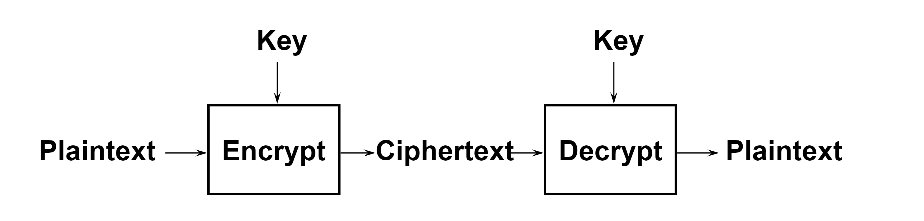
\includegraphics[scale=0.5]{images/1-symm_crypto.PNG}
	\caption{Symmetric encryption primitives.}
	\label{fig:sym_crypto}
\end{figure}

For a plaintext enrypted with key $K$, we write \{plaintext\}$_K$. The main challenge of symmetric cryptography is the distribution of the secret key (a confidential and authentic channel is required).

\paragraph{Stream / State Ciphers}
Plaintext digits combined with a pseudorandom cipher digit stream (keystream) to encrypt them one at a time with the corresponding keystream digit (typically with an XOR operation).

\paragraph{Keystream}
Utilize a pseudorandom generator (PRG) to generate a keystream from a seed.
E.g. Use shared key $k$ and initialization vector $IV$ for the seed, share cipher text and $IV$ (ciphertext = plaintext $\oplus$ PRG($k, IV$).

\paragraph{Initialization Vector / Nonce}
Pseudorandom fixed-size input to a cryptographic primitive. Best if non-repeating in repeated encryption applications.

\paragraph{One-Time Pad Stream Cipher}
Plaintext encryption using a one-time pre-shared key with the same size (or longer than) the message being sent. Impossible to break if: 1) key is truly random and 2) key is never (partially) reused.

\paragraph{ChaCha / Salsa Stream Cipher}
A 512-bit keystream is generated with a 256-bit key and a 64-bit nonce using add-rotate-XOR operations. %TODO: more on this?

\paragraph{Keystream Reuse Attack}
If $A$ and $B$ are same-length plaintexts encrypted with the same key $K$, we have (with $C$ being the key stream):

$$
\{A\}_K = A \oplus C \text{ and } \{B\}_K = B \oplus C
$$

$$
\{A\}_K \oplus \{B\}_K = (A \oplus C) \oplus (B \oplus C) = A \oplus B \oplus C \oplus C = A \oplus B
$$

Even without knowing $A$ or $B$ specifically, both plaintexts can be easily derived / analyzed.

\paragraph{Ciphertext Modification Attack}
Changing digits of the ciphertext will alter the corresponding values in the plaintext after decryption. Authenticity of ciphertext is required to defend against this attack.

\paragraph{Block Ciphers}
Blocks (fixed-length groups of bits, last block padding if needed) are encrypted using a symmetric key each (one-to-one mapping).
E.g. Advanced Encryption Standard (AES).

\paragraph{Mode of Operation}
Describes how to repeatedly apply a cipher's single-block operation to encrypt the data. There are two categories: confidentiality-only (ECB, CBC, CTR, etc.) and authenticated encryption (AE) that combines confidentiality and authenticity. Integrity protection is an entirely separate goal seen in AEAD only.

\paragraph{Electronic Code Book (ECB)} 
Natural approach - split plaintext into blocks and use the same key for each block. Has the disadvantage that equal blocks correspond to equal ciphertexts - lack of diffusion. ECB does not hide data patterns well (esp. in images with large areas of uniform colors).

\paragraph{Cipher Block Chaining (CBC)}
Apply XOR to each block with previous ciphertext before encrypting. Use an $IV$ for the first block. Each ciphertext block depends on all plaintext blocks processed up to that point. Cannot be parallelized and message must be padded to a multiple of cipher block size. Plaintext block can be recovered from two adjacent blocks of ciphertext (allows for parallelized decryption).

\paragraph{Counter Mode (CTR)}
Turn block cipher into a stream cipher. Generates the next keystream block by encrypting successive values of a counter (any function that does not repeat for a long time, e.g. increment by one counter). Use an $IV$ for the first block and increment for next blocks. Has the same vulnerabilities as any other stream cipher.

\paragraph{Authenticated Encryption}
Ensures confidentiality and authenticity of data.
E.g. Encrypt-then-MAC (EtM), Encrypt-and-MAC (E\&M), MAC-then-Encrypt (MtE).

\paragraph{Message Authentication Code (MAC)}
Cryptographic checksum for message authentication and integrity. Can only be calculated with a shared secret key (MAC$_K$(M)).

\begin{figure}[h]
	\centering
	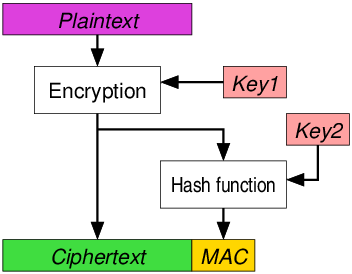
\includegraphics[scale=0.4]{images/1-EtM.png}
	\caption{EtM approach.}
	\label{fig:etm}
\end{figure}

\begin{figure}[h]
	\centering
	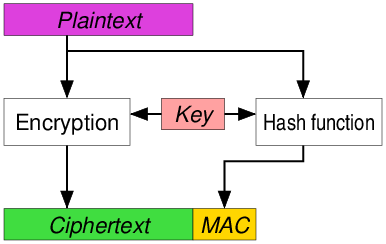
\includegraphics[scale=0.4]{images/1-EaM.png}
	\caption{E\&M approach.}
	\label{fig:eam}
\end{figure}

\begin{figure}[h]
	\centering
	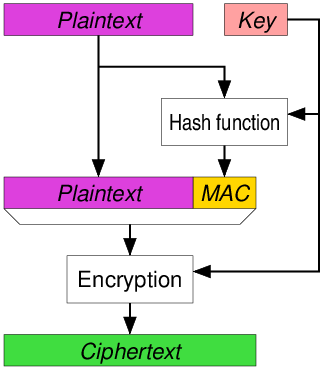
\includegraphics[scale=0.4]{images/1-MtE.png}
	\caption{MtE approach.}
	\label{fig:mte}
\end{figure}

\paragraph{Authenticated Encryption with Associated Data (AEAD)}
Allows a recipient to check the integrity of both the encrypted and unecrypted message (on top of confidentiality and authorization). Based on Encrypt-and-MAC (E\&M).

\paragraph{Galois Counter Mode (GCM)}
AEAD based on a block cipher in CTR mode (block size of 128 bits) and Galois MAC - mostly used with AES (AES-GCM). 

\begin{figure}[h]
	\centering
	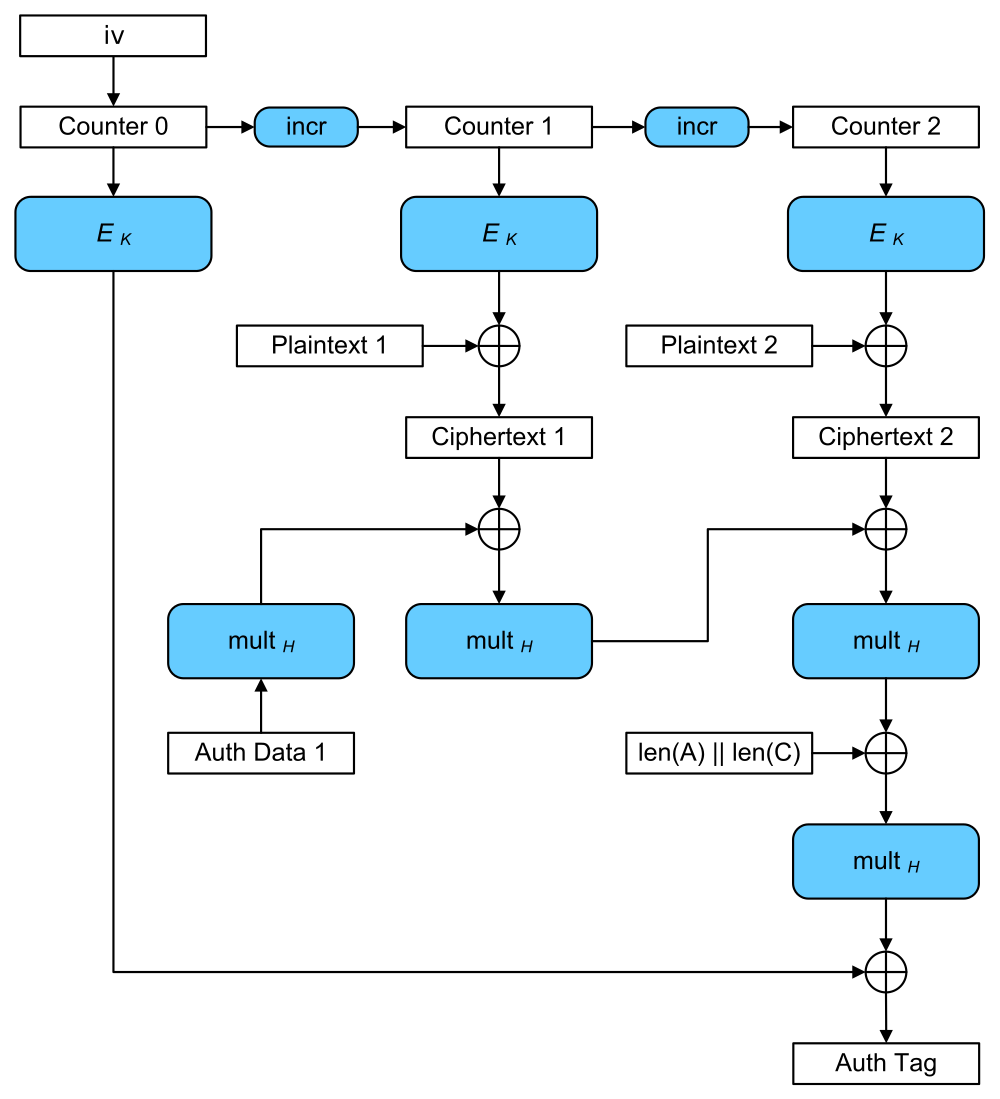
\includegraphics[scale=0.2]{images/1-gcm.png}
	\caption{GCM with only two plaintexts.}
	\label{fig:gcm}
\end{figure}


\subsubsection{Asymmetric / Public-Key Cryptography / PKI}

%TODO examples of key exchange

Cryptographic primitives using pairs of keys (public and private). The pairs are generated using cryptographic one-way functions. Can be used to establish a secret symmetric key.

Messages are encrypted using the receiver's public key and can only be decrypted with the receiver's private key. To ensure authenticity, a message can additionally be signed with the sender's private key and verified with their public key.

The main challenge is the authentication of the key (an authentic channel is required).

\paragraph{Diffie-Hellman Key Exchange}
A method to securely exchange a key over a public channel based on the discrete logarithm problem (see Figure \ref{fig:dhke}). Is susceptible to man-in-the-middle attacks in which attacker impersonates either receiver to each sender, resulting in two different established keys.

\begin{figure}[h]
	\centering
	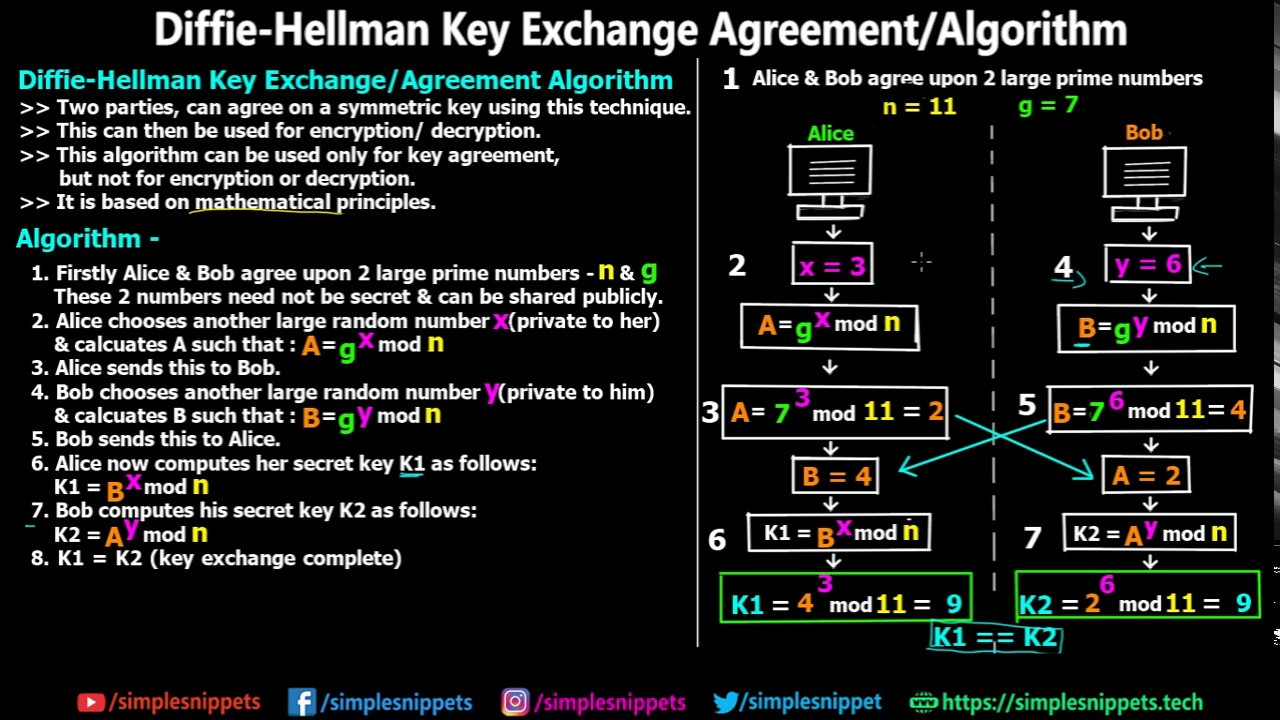
\includegraphics[scale=0.2]{images/1-diffie_hellman.jpg}
	\caption{Diffie-Hellman key exchange.}
	\label{fig:dhke}
\end{figure}

\paragraph{Discrete Logarithm Problem}
Given $x$, $g$ and $p$ find $a$ ($g^a$ mod $p = x$).

\paragraph{RSA Algorithm} Same as with Diffie-Hellman, just in a different way (see Figure \ref{fig:rsa}).

\begin{figure}[h]
	\centering
	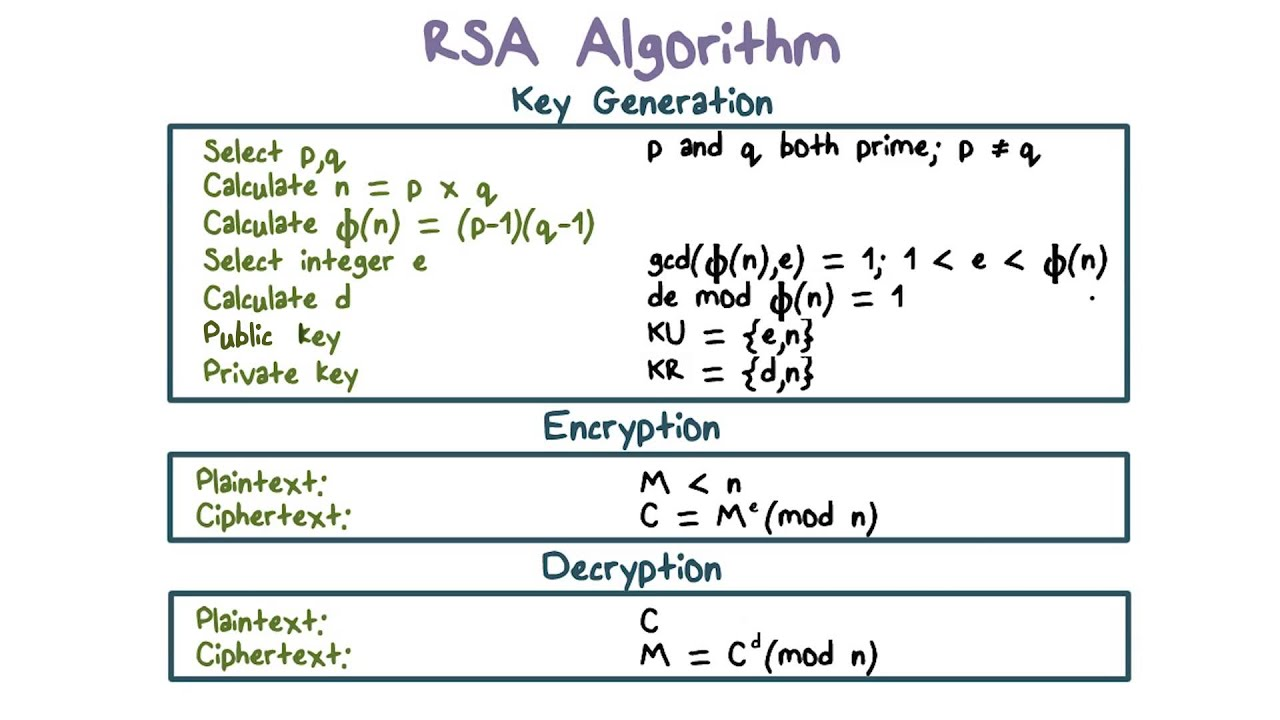
\includegraphics[scale=0.2]{images/1-rsa.jpg}
	\caption{RSA key generation and de/encryption.}
	\label{fig:rsa}
\end{figure}

\paragraph{Encrypted Key Exchange (EKE)}
Both ends share a password $P$ and want to authenticate each other along with establishing a shared secret key (see Figure \ref{fig:dh_eke}).

\begin{figure}[h]
	\centering
	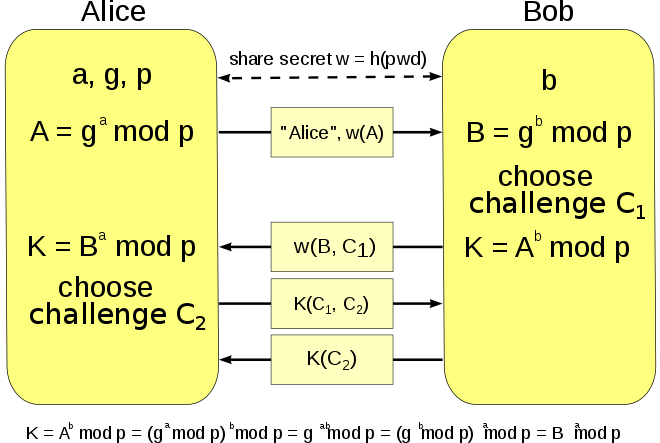
\includegraphics[scale=0.3]{images/1-dh_eke.png}
	\caption{DH-EKE scheme.}
	\label{fig:dh_eke}
\end{figure}

\paragraph{Authentication vs. Signature}
Authentication enables a receiver to verify the origin of a message, but it cannot convince a third party of the origin. A signature allows for the verification of origin and will convince a third party of it as well (a signature provides authentication).

\subsubsection{Hash Functions}

\paragraph{Cryptographic Hash Functions}
Map an arbitrary-length input into a finite length output with the following properties:

\begin{itemize}
    \item \textbf{One-way:} given $y = H(x)$, one cannot find $x'$ s.t. $H(x') = y$.
    \item \textbf{Weak collision resistance:} given $x$, one cannot find $x' \neq x$ s.t. $H(x) = H(x')$.
    \item \textbf{Strong collision resistance:} one cannot find $x' \neq x$ s.t. $H(x) = H(x')$.
\end{itemize}

They can be used for digital signatures, MACs and other forms of authentication. Also used for fingerprinting (unique IDs, no duplicates) and as checksums (check integrity). Most common cryptographic hash functions include MD5, SHA-1, SHA-2 and SHA-3.

SHA-1 is known for collision attacks. E.g. Git only uses SHA-1 value to identify commits - attacker can commit good code and distribute a repo version with bad code that has the same SHA-1 value.

%TODO add exercise 2.8 - calculation with hash collisions

\paragraph{One-Way Hash Chain}
A method to produce many one-time keys from a single key. Pick a random starting value and a public one-way hash function, continuously apply function to resulting values and use results in reverse order of construction. Allows for authentication of $r_i$ using $r_j$ where $j < i$ and $r_j = F(r_i)$.

\paragraph{Merkle Hash Trees (Binary Hash Chain)}
Efficient and secure verification of large data. Data is divided into blocks with each block labelled with its cryptographic hash value (leaf nodes). Every non-leaf node is the hash value of the concatenated hash values of its two children (if binary). To demonstrate that a leaf node is part of a binary tree, it is required to compute a number of hashes proportional to the log of leaf nodes - this allows for partial checking (as compared to hash lists where we would need the full file). Usually, the root hash received from a trusted source is compared to a hash tree from a potentially untrusted source.




%TODO: conversions and useful units





\subsection{Network Refresher}
%TODO esp. NAT, BGP, DNS


\newpage

\section{SSL/TLS Public Key Infrastructure}

\paragraph{Goal of TLS}
Achieve secure internet communication by preventing eavesdroppers from learning sensitive information and enabling entity and message authentication.

\paragraph{TLS Challenges}
\begin{itemize}
    \item No additional latency of contacting servers during TLS handshake.
    \item Keys should be immediately usable and verifiable after initial registration.
    \item Users should not be concerned with checking the legitimacy of a certificate.
    \item Covering the entire certificate life cycle.
\end{itemize}

%TODO: approaches to improve TLS and what's wrong with it, let's encrypt, ACME

\paragraph{Certificate Authority (CA)}
Entity (trusted third-party) that issues digital certificates, which certify the ownership of a public key by the uniquely named subject.

\paragraph{(Public-Key) Certificate}
The format of such certificates is specified by the \textit{X.509} or \textit{EMV} (proprietary - used for ATMs and the like) standard. Certificates can be revoked and renewed (challenge: consistency, availability and tolerance to partition - CAP theorem). 

Additionally to CA signed, certificates can be self-signed (changes the trust model, considered unsafe for public-facing services, suitable for internal sites or testing environments).

%TODO: examples, x.509

\paragraph{Trust Anchor / Root}
Self-signed certificates of public keys that are allowed to sign other certificates (trust assumed, not derived). One anchor can involve multiple entities. Involved in the whole chain of trust and used during certificate path validation (certificate hierarchy). With cryptographic operations, trust can be transferred from one entity to another.

Root certificates are only used to sign intermediate certificates since they need to be as safe as possible. Revoking even one of them can make many certificates invalid if they sign more. Roots are kept offline and used as rarely as possible.

\paragraph{PKI Alternatives}
If one of the many trusted CAs is compromised, security of all digital certificates is susceptible to attacks. One alternative architectures is Attack Resilient PKI (ARPKI). To impersonate a domain, a large number of entities need to be compromised. Another alternative is a web of trust = distributed PKI as seen in Pretty Good Privacy (PGP).

\paragraph{ARPKI}
%TODO

\paragraph{Web of Trust / PGP}
Decentralized PKI where users establish direct trust with each other (private and public key system). Indirect trust to a destination can be established by trusting someone that directly trusts destination. There are no CAs and therefore no single point of failure stemming from a compromised CA hierarchy.

PGP uses this model to provide cryptographic privacy and authentication for data communication. It is used for signatures and encryption.
%TODO: more

\paragraph{Trust Agility}
The ability for the user to choose which entities to trust. User can also specify to require additional certification for entities not covered by chosen group of trust anchors.

\paragraph{Levels of Trust}
\begin{itemize}
    \item \textbf{No SSL/TLS:} domain/website served via HTTP.
    \item \textbf{Domain Validation (DV):} site is secure, not necessarily the entire business.
    \item \textbf{Organisation Validation (OV):} CA carries out some vetting of the organisation (verify existence of company and domain name, verification phone call, etc.)
    \item \textbf{Extended Validation (EV):} CA undertakes comprehensive vetting process of the organisation (verify legal and physical existence of organisation, identity matches official records, exclusive rights to the domain, etc.).
\end{itemize}

\paragraph{HTTP Strict Transport Security (HSTS)}
Allows web servers to declare that browsers / user agents should automatically interact with it using only HTTPS connections. HSTS helps to protect websites against MITM-attacks (i.e. protocol downgrade, cookie hijacking = stealing session keys in HTTP, etc.).

\paragraph{HTTP Public-Key Pinning (HPKP) (deprecated)}
Allows HTTPS websites to resist impersonation by attackers using misissued/fraudulent certificates. A set of hashes of public keys valid for a given time is delivered to the client (web browser) which must appear in the certificate chain of future connections to the same domain name. During their validity time, a client expects to see one or more of those public keys in its certificate chain.

Since HPKP is trust on first use (TOFU), meaning the provided hashes are trusted, it can still be susceptible to a MITM attack if the first policy received comes from an attacker. Furthermore, weak hashes allow for easy collisions.

Careful: when renewing the certificates for a domain, new hashes (with a new age) have to be distributed to not DoS oneself.

\paragraph{Online Certificate Status Protocol (OCSP)}
Protocol to obtain the revocation status of an X.509 certificate - an alternative to certificate revocation lists (CRL). OCSP responders (servers) respond to requests to verify the status of a certificate to check if it is still valid. Vulnerable to replay attack where an attacker captures the "still good" response and replays it at a later time where the certificate might already be revoked.

\paragraph{OCSP Stapling}
Standard for checking the revocation status of X.509 digital certificates. The presenter of a certificate can bear the resource cost involved in providing OCSP responses by appending (= stapling) a time-stamped OCSP response signed by the CA to the initial TLS handshake - eliminating the need for the client to contact the CA.

Original OCSP introduced a significant cost for CAs because they have to respond to numerous OCSP requests. Furthermore, privacy issues were introduced with the need to contact a third-party and not receiving a response can be annoying.

\paragraph{DNS-Based Authentication of Named Entities (DANE)}
Protocol to bind X.509 certificates to domain names using Domain Name System Security Extensions (DNSSEC). Allows to authenticate TLS entities without a CA. %TODO: use cases?

\paragraph{Certificate Transparency (CT)}
A standard for monitoring and auditing digital certificates. It creates a system of public logs recording all certificates issued by publicly trusted CAs. This allows for efficient identification of mistakenly / maliciously issued certificates (which is usually very slow). Makes it impossible for a certificate to be issued for a domain without the domain owner knowing.

In a CT log, new certificates are appended to an ever-growing signed (by log server) Merkle Hash Tree. Each appended certificate must have a valid signature chain. Monitors (CAs) check the log servers for misbehavior and request the addition of a newly issued cert. Auditors (clients) verify certificate existence by checking the log servers and exchange info with the monitors on the log server status (to ensure that it is not compromised).

Certificates stay on the log forever (even revoked ones). Merkle Tree insertions are easy but immediate deletion is not. System might implement revocation transparency.

Often used together with OCSP stapling in which a certificate presenter has to add certificate to a public log and the CT log signature needs to be stapled to signature.

%TODO: more on this, watch lecture, exercise 2!






\newpage

\section{More on TLS}

\subsection{TLS Overview}

\paragraph{High Level Goals}
TLS aims for security in face of an attacker with complete control of the network. The only requirement for the underlying transport is a reliable and in-order data stream (TLS is between the transport and application layer).
\begin{itemize}
    \item \textbf{Entity Authentication:} Server side is always authenticated, client side optional. Authentication via asymmetric crypto (signatures) or symmetric pre-shared key (unique for each session).
    \item \textbf{Confidentiality:} Data only visible to the endpoints, but TLS does not hide length of data (padding possible).
    \item \textbf{Integrity / Reliability:} Data cannot be modified without detection. Guarantees also cover reordering, insertion and deletion.
\end{itemize}

\paragraph{Part 1: Handshake Protocol}
Used by client and server to negotiate cipher suite\footnote{Click \href{https://ciphersuite.info/cs/}{link} for a list of all 337 cipher suites and their security status.} (set of algorithms to secure the connection, e.g. key exchange, encryption, MAC, etc.), authenticate each other (certificates and public keys) and establish session keys used in the Record Protocol (see below).

\paragraph{Establishing Session Keys}
The client either encrypts a random number with the server's public key, with which both parties generate a unique key or the client uses a Diffie-Hellman key exchange (see previous Section). The second option has the property of forward secrecy.

\paragraph{Forward Secrecy}
Future disclosures of encryption keys cannot be used to decrypt communications recorded in the past. More specifically. session keys cannot be compromised even if long-term secrets used in the session key exchange are compromised. Additionally, compromising unique session keys should not affect any other communications encrypted with a different session key. Assumes passive attacks, i.e. does not protect against an active MITM attack.

E.g.: In HTTPS, the long-term secret is typically the private signing key of the server.

\paragraph{Part 2: Record Protocol}
Using the session keys established in part 1, the application layer communication is guaranteed to be confidential and reliable. 

The Record Protocol provides a stream-oriented API (fragmentation/coalescence of data allowed). A record is a TLS data unit, which is a fragment of the data stream.

\paragraph{Cryptographic Protections in the Record Protocol}
\begin{itemize}
    \item Data origin authentication.
    \item Data integrity using a MAC.
    \item Data confidentiality using a symmetric encryption algorithm (integrity and encryption combined in TLS 1.3 by use of AEAD).
    \item Prevention of reflection attacks by key separation (different symmetric keys in different directions).
\end{itemize}

\paragraph{Reflection Attack}
Attacking a challenge-response authentication system that uses the same protocol in both directions by tricking the target into providing the answer to its own challenge.

\paragraph{TLS 1.0 (1999)}
First version of TLS (after migrating from SSL) and deprecated in 2020 due to security flaws.

\paragraph{TLS 1.1 (2006)}
Fixed the security flaws of version 1.1, such as protection against cipher-block chaining attacks.

\paragraph{TLS 1.2 (2008)}
Changed hash algorithms used for the protocol, enhanced cipher suite negotiation abilities between client and server, support for authenticated encryption ciphers (see AE(AD)), addition of AES cipher suites, etc.
In 2011, backward compatibility with SSL was removed to prevent version fallback.

\begin{figure}[h]
	\centering
	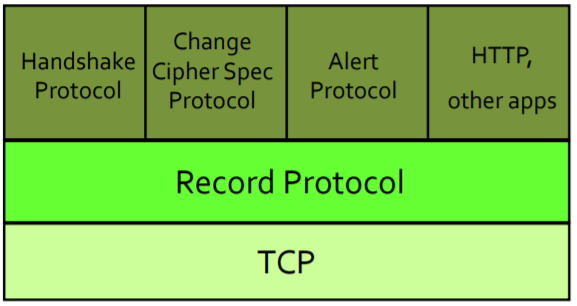
\includegraphics[scale=0.4]{images/3-tls12.PNG}
	\caption{TLS 1.2 protocol architecture.}
	\label{fig:tls12}
\end{figure}

\paragraph{TLS 1.2 Handshake}
When using TCP, the full handshake is a 3-RTT protocol (see Figure \ref{fig:poorhandshake}). 

\begin{figure}[h]
	\centering
	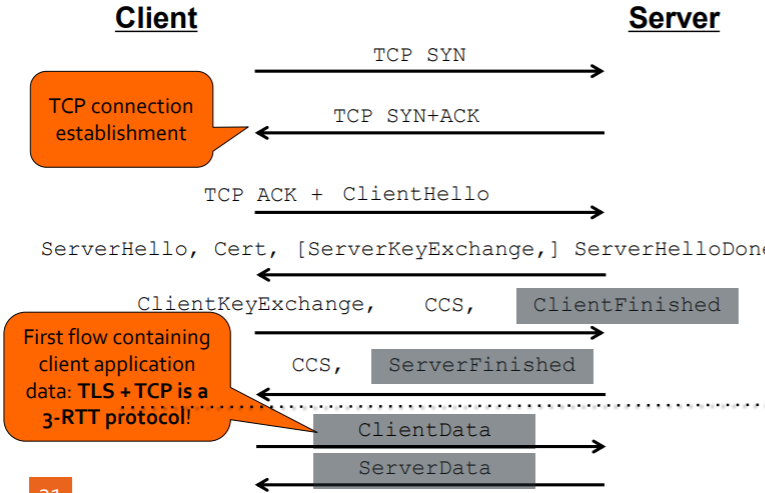
\includegraphics[scale=0.5]{images/3-poorhandshake.PNG}
	\caption{The full TCP + TLS 1.2 handshake.}
	\label{fig:poorhandshake}
\end{figure}

\paragraph{TLS 1.3 (2018)}
Not yet widely used. Significant change to the way of coordinating the cipher suites between machines (part of the Handshake Protocol) by reducing the number of messages needed (cannot be used for version 1.2 and vice versa - the numbers of suites is reduced from 337 to 5). The key agreement and authentication algorithms are separated from the cipher suites. Mandates forward secrecy. Also removed support for less secure algorithms and introduced further security measures. Dropped support for insecure obsolete features such as compression (enabled \textit{CRIME} attack), renegotiation, non-AEAD ciphers (previous versions support MtE), etc. Encrypts all handshake messages after the \textit{ServerHello}.

TLS 1.3 basically wants to mimic QUIC by achieving the same RTT profile (excluding TCP overhead since it is unavoidable for TLS). QUIC offers a native 1-RTT handshake and a 0-RTT mode.

Compared to previous versions where the complete handshake is in the clear, version 1.3 encrypts almost all handshake messages with a separate key, providing security to both passive and active attacks on both ends.

\begin{figure}[h]
	\centering
	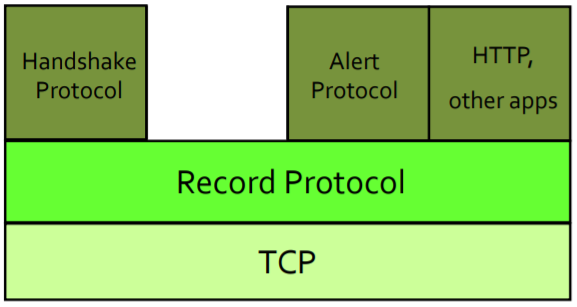
\includegraphics[scale=0.4]{images/3-tls13.PNG}
	\caption{TLS 1.3 protocol architecture.}
	\label{fig:tls13}
\end{figure}

\paragraph{Datagram TLS (TLS over UDP)}
Prevents eavesdropping, tampering or message forgery of UDP connection. Has to deal with fragmentation and packet reordering / loss. Avoids the \textit{TCP meltdown problem} when being used to create a VPN tunnel \footnote{\href{http://sites.inka.de/bigred/devel/tcp-tcp.html}{\textit{Why TCP over TCP Is A Bad Idea}}}.

\subsection{TLS 1.3 Details}

\paragraph{TLS 1.3 Record Protocol}
Each fragment is encoded into payload, ctype (single byte representing content type, i.e. handshake message, alert message or application data) and optional padding (used to hide true length of fragments). Encoded fragments are then encrypted using AEAD and appended to a record header.

For the AEAD encryption, a nonce is created by XORing the SQN and an IV. The 64-bit sequence number (SQN) is incremented for each record sent on a connection and maintained at each end of the connection (not included in header). The IV is a fixed per-TLS connection pseudorandom value derived from secrets established during the Handshake Protocol. XOR (masking) ensures that the nonce sequence is unique for each connection. This facilitates analysing security in a multi-connection setting.

The record header contains a 1-byte dummy type field, a 2-byte legacy version field (negotiated during handshake) and the length of the AEAD ciphertext (2 bytes).

AEAD-decryption failures are fatal and will lead to the connection being torn down and the key material being thrown away.

\paragraph{Attacks not Prevented by TLS 1.3 Record Protocol}
\begin{itemize}
    \item Truncation attacks on the stream of records.
    \item Application layer confusion.
    \item Timing attacks on the padding scheme.
\end{itemize}

\paragraph{TLS 1.3 Handshake Protocol}
Full handshake in 1 RTT (compared to 2 in 1.2 and earlier resp. 3 if TCP is counted. Achieved by only ever doing DH (elliptic or finite-field) and client speculatively sending several DH shares in supported groups (only a few) - server then picks one, replies with its share and Record Protocol keys can be derived. When resuming a previously established connection, a 0-RTT handshake is possible since shared state is kept with which a PSK can be derived. TLS 1.2 and earlier had the complete handshake in the clear, 1.3 encrypts almost all handshake messages and derives separate key to protect them (security for passive and active attacks).

%TODO DH shares, groups and curves? continuity

%TODO print out the slides for this part


\paragraph{Future of TLS}
%TODO: important? concluding remarks? largest security shifts


%TODO overview comparison to older versions? esp. handshake



\newpage

\section{IPv6 Security}

\paragraph{Address Space}
IPv6 uses 128-bit addresses, which theoretically allows for $2^{128}$ unique addresses. An address is represented as eight colon-separated groups of four hexadecimal digits (can be shortened by excluding the zeroes, e.g. \textit{2001:db8::8a2e:370:7334}).

\paragraph{Link-Local Address}
An address that is only valid for communications within the network segment/broadcast domain that a host is connected to. In IPv6, they are assigned from the block \textit{fe80::/10} (prefix, with a 64-bit suffix computed by host itself) and every host is required to have at least one / one for each network interface. An LLA is unique in the LAN (also named unique local address, ULA). LLAs can be tranlated to global addresses using a NAT.

To not leak any information, LLAs do not embed the host's MAC address anymore and are instead generated via algorithms using some kind of randomness. Knowing a MAC address allows for physical attacks.

\paragraph{Link-Layer Addresses} To map IP to MAC addresses, IPv6 uses the Neighbor Discovery Protocol (NDP) instead of ARP, since it does not support the broadcast addressing method. Nodes using the requested IP address respond to neighbor solicitation messages originating from an asking host with their link-layer addresses.

This has the potential for a DoS attack by overflowing a host's buffer or overwriting real entries.

\paragraph{Router Solicitation}
By sending a multicast ICMPv6 router solicitation message to the all-routers group, a host learns about the network from neighbouring routers (router advertisement) and can establish a globally unique address with an appropriate unicast network prefix. Router advertisements also include further information, i.e. if and how DHCP should be used by the host.

\paragraph{Duplicate Address Detection (DAD) DoS}
Hosts use DAD to assign themselves unique LLAs. To ensure they are unique, hosts ask all nodes of a LAN if the address is already in use. This allows for an easy DoS by simply replying that the address is already in use to each DAD request.

\paragraph{Shadow Networks}
Data flowing through new IPv6-enabled connections and onto the existing IPv5 network while the IPv4 security in place is unable to identify this new type of traffic (e.g. traffic is not subject to firewall rules, etc.). This is a problem if a network admin is not aware of new IPv6 ability.

In general, IPv6 connectivity cannot be prevented as long as a node is part of a bi-directional communication. Such a channel can be used as a tunnel.

\paragraph{Tunneling}
The act of encapsulating IPv6 packets in IPv4 packets to allow for IPv6 connectivity anywhere. Not used much.

E.g.: \textit{Teredo}, \textit{6to4}, etc.

\paragraph{Injecting IPv6 Addresses}
In a LAN without an IPv6 router, a host could be made to act like one. All IPv6 capable hosts automatically assign themselves an IPv6 address. With this, the host can easily enact a MITM attack and bypass any IPv4 firewalls (via tunneling).

If a LAN already hosts IPv6 routers, one can simply setup a router with a higher priority since router advertisements include a priority field.

Such rogue router advertisements can be prevented via filtering (RA and DHCPv6 messages).

\paragraph{Multicast Groups}
IPv6 does not implement IP broadcast with a special broadcast address. Using multicast groups, a message can be broadcasted to all link-local nodes (\textit{ff02::1}) or all link-local routers (\textit{ff02::2}).

\paragraph{Filtering}
%TODO: ?

\paragraph{Fragmentation Attack}
IPv4 fragments packets, requiring routers to store and/or re-assemble packets. By sending bogus or overlapping fragments, a router can crash (memory exhaustion). IPv6 does not support fragmentation in the network - the work is shifted to the end hosts (routers return ICMP6 messaged indicating that a packet is too big).

\paragraph{Internet Protocol Security (IPsec)}
Authentication and encryption of IP packets (mainly used for VPNs). Part of the IPv6 specification but not implemented in practice (too complex (NATs), other methods of security) - only a recommendation.

\paragraph{NAT Is Not Security (NINS)}
NAT maps IP addresses 1:1 / 1:n or to protocol ports (PNAT). It is not to be used as a (stateful) firewall, since access from outside is possible if the table entries are known. %TODO: more on NAT vs. firewall?

\paragraph{Conclusions}
\begin{itemize}
    \item IPv6 is not more or less secure than IPv4.
    \item Attacks are similar to the ones on IPv4.
    \item Networks need to be prepared to handle IPv6 to avoid security holes.
\end{itemize}
\newpage

\section{Virtual Private Networks}

\subsection{Overview}

\paragraph{VPN}
A VPN creates a secure channel between two private networks over an untrusted, public network (the Internet) - this provides security on the link / network layer. Additionally, functionality and management of the private network can be transferred to the established VPN.

A VPN can connect physically separated networks (site-to-site), connect a remote host to a company/university network (host-to-site), circumvent censorship, avoid tracking, hide user's IP address, spoof locations, allow access to restricted content, etc.

A VPN provider has access to metadata of all traffic - anonymity is not given.

\paragraph{Part 1: Set-Up Phase}
The tunnel endpoints authenticate each other and set up keys (similar to the TLS handshake).

\paragraph{Part 2: Tunneling Phase}
Packets are encapsulated and decapsulated at the endpoints. Additionally, the original data is encrypted and authenticated with a MAC.

\paragraph{VPN Tunnel Properties}
A VPN tunnel holds similar security properties as the TLS Record Protocol (source authentication, data integrity, confidentiality, replay suppression, etc.). However, some tunneling protocols do not provide encryption/authentication.

\paragraph{VPN vs. TLS}
\begin{itemize}
    \item VPN protects all kinds of traffic (e.g. DNS requests, etc.).
    \item Services in private networks / behind firewalls can be accessed with VPNs.
    \item VPN data is only secure in the tunnel. TLS protects data end-to-end.
    \item VPN servers can see unencrypted traffic (here, TLS is still necessary).
    \item A web server cannot be authenticated with VPN, only the tunnel endpoint.
    \item TLS does not authenticate clients.
    \item VPN utilize many different protocols.
    \item TLS is commonly used on top of a VPN.
\end{itemize}

\paragraph{Performance / Availability}
VPNs introduce overhead with additional cryptographic operations, potential detours and limited bandwidth at VPN servers. There is no built-in defense against (D)DoS and routing attacks, therefore VPNs do not provide a higher availability. Packet filtering targeting VPN packets would need to target all VPN packets since content is hidden.

\paragraph{VPN vs. VLAN}
A VPN connects two different networks, resulting in one virtual network over multiple physical ones. VLANs set up multiple isolated virtual networks (logical groupings) on a single physical infrastructure. VLANs are often used in cloud-computing environments to isolate communication between VMs or to form multiple broadcast domains in a network with frequent broadcasts. VLANs do not provide authentication. A virtual extensible LAN (VXLAN) combines both features.

VLANs are L2 constructs, analogous to IP subnets which are L3 constructs. There is often a one-to-one relationship between a VLAN and an IP subnet (it is possible to have multiple subnets on one VLAN).

\paragraph{Implementing VPN Functionality}
There are many different protocols and applications that implement VPN functionality. They can differ in authentication mechanisms (PSK, PKI, etc.), the tunnel protocol (custom ones, SSTP, etc.), the inner protocol = outermost header of an encapsulated packet (network vs. link layer VPN - e.g. IPsec L3, WireGuard L2, etc.) and of course how they're implemented (in user space, a kernel module, directly in hardware, etc.).

\paragraph{Endpoints at Hosts}
A VPN creates virtual network adapters (e.g. "eth2", "tun0", etc.) at the end hosts, one route with the public IP of the VPN server as a destination and a new default route to the private address of the VPN tunnel. They can be used like any other network adapter and one can either send all traffic through it or selectively (\textit{split tunnel}) by choosing only a subset of IP prefixes that should use the VPN. %TODO image? see notes


\subsection{VPN Implementations}

\paragraph{IPsec}
IPsec is a secure network protocol suite (very large, many options / modes) that authenticates and encrypts packets over an IP network - also supports data integrity and replay protection. There is mutual authentication between agents at the beginning of a session along with negotiation of keys to use during it. Problems include difficult configuration due to many options where some don't even provide security (no encryption and no authentication) and the possibility of insecure ciphers (similar to TLS problems).

\textbf{Comparison to TLS:} In HTTPS, client certificate authentication is rare while in IPsec it is the norm. This is because websites are usually publicly accessible while private networks apply strong restriction on authorized users. IPsec explicitly includes sequence numbers in its packets since IP is only best-effort (loss, reordering, duplication) while TLS maintains only local counters since it runs on top of TCP.


\begin{figure}[h]
	\centering
	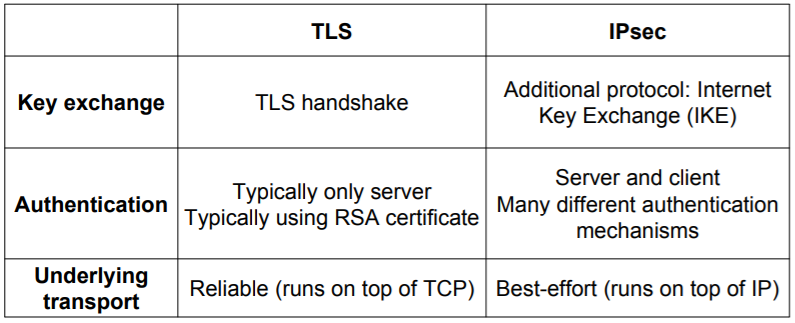
\includegraphics[scale=0.6]{images/5-ipsec_tls.PNG}
	\caption{Comparison of TLS and IPsec.}
	\label{fig:ipsec_tls}
\end{figure}

\textbf{Typical Session:} first set up a security association (SA) via Internet Key Exchange (IKE) and then encapsulate packets and tunnel them between SA endpoints with Encapsulation Security Payload (ESP).

\textbf{IKEv2:} first establish a temporary and anonymous key for the rest of the IKE exchange and then authenticate each other by sending identity, (certificate), sig (asym.) / MAC (sym.), etc. (see Figure \ref{fig:ike}). Passive attacks cannot uncover the identities but an active MITM attack might. In case of ephemeral DH values at the beginning, we have perfect forward security. %TODO: how exactly?

\begin{figure}[h]
	\centering
	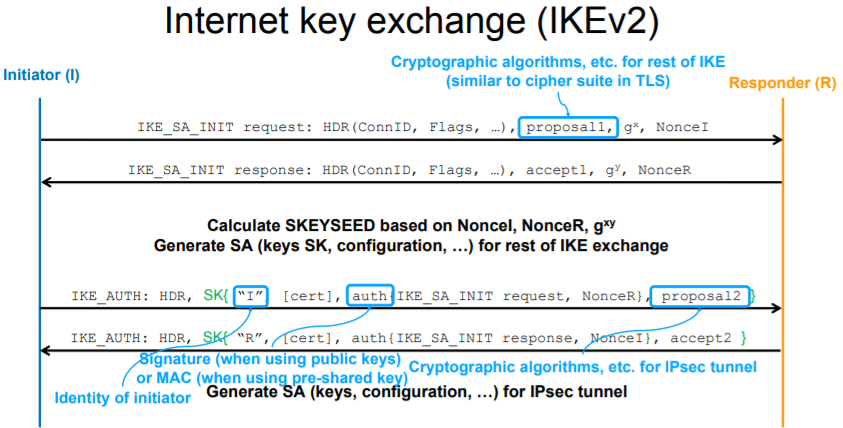
\includegraphics[scale=0.7]{images/5-ike.PNG}
	\caption{Simplified overview of the IKEv2.}
	\label{fig:ike}
\end{figure}

\textbf{ESP:} the original IP packet is first padded with the ESP trailer that also includes the type of the original packet (appended at the end). It is then fully encrypted. Then, the ESP header is added which includes the SA identification and a sequence number (replay protection, nonce for certain encryption algos, etc.). Lastly, an Integrity Check Value (ICV) is created and appended at the end - it is a MAC over the entire packet. Finally, a new IP header is added.

\textbf{Other Options:} there can be additional messages in IKEv2 (EAP, cookies, etc.) and other modes like the transport mode for end-to-end connections or an Authenticated Header (AH) protocol instead of ESP if we only want authentication but no encryption.

\paragraph{WireGuard}
Much faster and smaller than other options (IPsec, OpenVPN, etc.) by removing cryptographic agility, i.e. only support chosen state-of-the-art primitives (single cipher suite) s.t. negotiation is simplified and insecure primitives are removed. Configuration is kept simple. Attack surface is minimal by keeping the codebase small (also makes formal verification easier). L3 packets are encapsulted and transformed into L4 UDP only packets.

\textbf{Key Exchange and Authentication:} the WireGuard handshake follows the Noise Protocol Framework built exclusively on elliptic-curve DH exchanges. First, each peer has a static key pair (public and private) and specify in configuration which public keys are authorized. Each peer then creares an ephemeral key pair (public and private). The symmetric keys are then derived from four DH combinations (two static public key and two ephemeral public keys). See Figure \ref{fig:wireguard}. Since WireGuard is connectionless, a series of timers (based on message counts and time) are used to steer handshakes, key renegotiation and session termination. Perfect forward security is guaranteed with strict key rotation timers and the ephemeral ECDH session key exchange.

\begin{figure}[h]
	\centering
	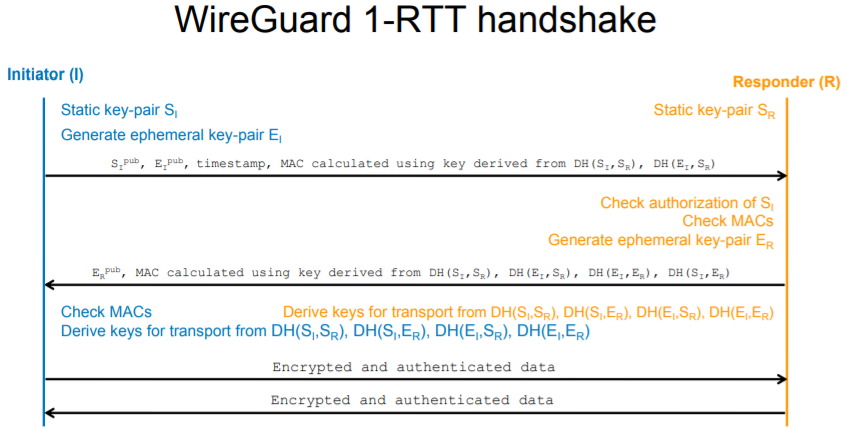
\includegraphics[scale=0.7]{images/5-wireguard.PNG}
	\caption{Simplified overview of the WireGuard handshake.}
	\label{fig:wireguard}
\end{figure}

\textbf{DoS Protection:} When under load, WireGuard can choose to respond with a cookie instead of processing the handshake (expensive cryptography). With this cookie, the initiator uses it as a key for computing HMACs of their message (similar to IKEv2 cookie-mode). Difference to IKEv2 cookie-mode is that an additional MAC is required on the handshake message (responder public key as HMAC key). Responder can stay completely silent unless initiator knows its public key. %TODO DoS protection in WireGuard and IPsec

%TODO if time, look at these
\paragraph{Point-To-Point Tunneling Protocol (PPTP)}

\href{https://citeseerx.ist.psu.edu/viewdoc/download?doi=10.1.1.503.7298&rep=rep1&type=pdf}{Comparison PPTP, L2TP, IPsec, etc.}

\paragraph{Generic Routing Encapsulation (GRE)}

\paragraph{Layer-2 Tunneling Protocol (L2TP)}

\paragraph{OpenVPN}

\paragraph{Secure Socket Layer (SSL)}

\paragraph{Secure Socket Tunneling Protocol (SSTP)}




\subsection{Summary}

\begin{itemize}
    \item VPNs create secure channels on the network/link layer.
    \item VPNs and end-to-end security (TLS) complement each other.
    \item There are many different VPN protocols and applications.
\end{itemize}
\newpage

\section{Wireless LAN}

%TODO own additions? from SOWN?

Guest lecture, more just experiences with it. 
\newpage

\section{Anonymous Communication Systems}

\subsection{Overview}

\paragraph{Sender Anonymity}
Adversary knows / is receiver and may learn messages. The sender is unknown but provides a return address / token.

\paragraph{Receiver Anonymity}
Adversary knows / is sender and may choose the messages. The receiver is unknown and receives data via a hidden service (pseudonym is known).

\paragraph{Sender / Receiver Anonymity Set}
Set of all individual senders / receivers indistinguishable from the real sender / receiver. The smaller the set, the less anonymity.

\paragraph{Unlinkability}
Adversary knows senders and receivers but not the link in between. Multiple users need to be communicating for this to work. Anonymity results in unlinkability.

\paragraph{Unobservability}
Adversary cannot tell whether any communication is taking place. For wireless, use methods like DSSS. For wired, constantly send traffic. Unobservability results in anonymity.

\paragraph{Plausible Deniability}
Adversary cannot prove that any particular individual was responsible for a message / any action. Anonymity results in plausible deniability.

\paragraph{Thread Model(s)}
An adversary may have:
\begin{itemize}
    \item Various degrees of control (local / global).
    \item Various types of (combinations of) control (network, compromised infrastructure, etc.). However, the infrastructure is never fully compromised.
    \item Passive or active behavior.
\end{itemize}
This results in unclear guarantees since the thread model is often not clearly specified.

\subsection{Mechanisms for Anonymous Communication}

\begin{itemize}
    \item \textbf{Broadcast:} for wireless communication, guaranteed receiver anonymity. However, a sender can be de-anonymized via triangulation. Use DSSS if the destination is trusted.
    \item \textbf{Hijacked Connections:} using a burner phone or hacking a WiFi connection to impersonate an ID.
    \item \textbf{Proxy / VPN:} to hide content from a proxy, use layered encryption. Problems: proxy can see metadata and may be a single point of failure. Use a cascade (onion) of multiple proxies (each proxy only sees addresses of two neighbors, works as long there is one honest proxy, message / forwarding info is encrypted multiple times).
\end{itemize}

\paragraph{Mix-Nets}
To obscure in- and outgoing messages, each proxy performs batching (collecting several messages and forwarding them if specific threshold is met). Additionally, proxies should change the order of the messages (mix). All messaged need to be padded to a fixed length to make them indistinguishable.

Vulnerable to intersection attacks. Since users often only communicate with a small subset of other users, an adversary can register the sets of destinations each time a message is seen,i.e. long term correlation attack (also possible with inter-packet intervals). More effective attack: statistical disclosure.

Return addresses are prepared by senders to receive replies. Senders know what keys will be established with each threshold mix proxy.

Problem: high latency, bad for web browsing - see Onion routing below. Forward security is not guaranteed.

\paragraph{Cover / Dummy Traffic}
Achieves full unobservability and prevents statistical disclosure attacks both for sending and receiving. A receiver regularly tries to retrieve messages from a threshold mix proxy and downloads it if there is any, else dummy message is returned. Not possible on Onion Routing.

\paragraph{Onion Routing / Circuit-Based Anonymity Networks}
No batching and mixing and no cover traffic, only layered encryption. Onion routing is flow-based, a virtual circuit / tunnel (keys) is established once per flow using only symmetric key crypto and each packet is forwarded by relays (proxy nodes). This has a lower anonymity guarantee than the previously introduced mechanisms. Also, the threat model is constrained - we can only deal with local adversaries that cannot launch confirmation attacks.

A sender remains anonymous because each intermediary knows only the location of the immediately preceding and following nodes. Only the final node knows its location in the chain, others don't know if they're the first or immediate ones.

\textbf{Circuit setup:} 

\textbf{Direct circuit setup:} 

\textbf{Telescopic circuit setup:} 

\textbf{Data forwarding:} 

\textbf{Circuit teardown:}

For all points above, see extra notes.

\paragraph{Mix-Nets vs. Onion Routing}
\begin{itemize}
    \item \textbf{Forwarding System:} message-based vs. circuit-based.
    \item \textbf{Layered Encryption:} asymmetric vs. symmetric.
    \item \textbf{Forward Security:} no vs. yes in case of the telescopic setup.
    \item \textbf{Latency:} high vs. low / medium.
    \item \textbf{Guarantees:} strong vs. attacks possible for strong adversaries.
\end{itemize}

\subsection{Attacks on Circuit-Based ACS}

Traffic-analysis attacks (confirmation attacks), e.g. flow / website fingerprinting, and higher-layer attacks, e.g. stack fingerprinting.

\paragraph{Passive Traffic Analysis}
Adversary observes edges of the network and records traffic patterns (flow length, bandwidth pattern, inter-packet timings). If measurements at two ends are similar / the same, an attacker could conclude that they are communicating. Real-time detection is challenging, more common to store and compare later (large storage needed).

\paragraph{Active Traffic Analysis}
Adversary actively modifies inter-packet timings (delaying / reordering packets). Packet drops possible but often detectable. If the clearly visible change is detected at the other end, attacker can conclude that they are communicating.

Flow watermarking: inject one bit of info (marked or not). Flow fingerprinting: inject multiple bits (e.g. sender IP address) to make the detection of correlation even easier. 

This requires a very strong attacker that controls the incoming traffic to a anonymous network (and can observe the outgoing traffic as in the passive case).

\paragraph{Website Fingerprinting}
Adversary needs only one observation point (ISP, other WiFi user, etc.). By building a database of fingerprints of websites (how many packets are send from each website), the fingerprints can be compared to the observed traffic patterns and the attacker can conclude which websites were accessed. Particularly effective for interactive applications such as health / tax forms. 

\paragraph{Traffic Analysis Resistance}
To resist such traffic analysis attacks, one could combine cover traffic and mixing (as mentioned above). Unfortunately, this introduces a significant overhead and is difficult to scale (large volumes of dummy traffic required). Such methods are only suitable for few applications (e.g. VoIP) with low bandwidth. To be really secure: restrict set of flow duration and bandwidth combination.

\paragraph{Higher-Layer Attacks}
Instead of observing / comparing / manipulating traffic, an attacker can observe information leaked from the protocols used, e.g. an end-to-end TCP might leak information due to the way the sequence numbers are chosen, how header fields are set, congestion control mechanisms, etc. This either requires packet inspection or being a malicious receiver.

A possible solution is to replace an end-to-end TCP connection with per-hop TCP connections.

HTTP / TLS fingerprints are in most cases unique (OS, browser type, languages, timezone, etc.). See amiunique.org/fp. To protect: either randomize the fingerprint each time a user is accessing the web or make them all look the same (uniformity - as in TOR).

Normally, a de-anonymization attack is done in other ways by, for example, tricking a user into downloading malware / files accessing Internet directly, analysing user behavior (e.g. text written in an online forum). To be anonymous, each layer (even human layer) has to be anonymized since any gap will break it entirely (unlike any other security properties).



\subsection{Tor: Second Gen Onion Router}

See extra notes.

\textbf{Additional features:} 

\textbf{Tor cells:}

\textbf{Example circuit setup:}

\textbf{Circuit extension:}

\textbf{Hidden services:}

\textbf{Directory authorities:}

\textbf{Censorship resistance:} 


\subsection{Summary}

\begin{itemize}
    \item You cannot be anonymous on your own (anonymity set).
    \item Anonymous communication is enabled by multiple relays and layered encryption.
    \item Mix-nets vs. circuit-based systems.
    \item Anonymous communication can be used for both good and bad purposes.
\end{itemize}




\newpage

\section{Border Gateway Protocol}

\subsection{Overview}

\paragraph{BGP} An exterior gateway protocol designed to exchange routing and reachability information among autonomous systems (AS) on the Internet (update messages over TCP). Routing decisions are made based on paths (list of ASes) and network policies / rule-sets configured by a network admin. For routing within an AS, see the Interior BGP (iBGP). %TODO: slides 43-55 for details

\paragraph{Path-Vector Routing Protocol} A routing protocol that maintains the received path information and updates it dynamically. Each entry of a routing table contains the destination network, the next router and the path to reach the destination.

In BGP, border routers (eBGP peers) send path-vector messages (over TCP) to advertise the reachability of networks. Each router verifies the received advertisements according to its policy.


\subsection{Security of BGP}

\paragraph{BGP Hijacking} BGP routers accept advertised routes from other BGP routers by default (automatic and decentralized routing). This allows for accidental or malicious disruption (blackhole, redirection, interception) by taking over an entire IP prefix(es) ($\approx$ AS) and illegitimately advertise for it. A stronger variation is to originate a more specific (longer) prefix fitting the victim's address space. Traffic will follow the longest matching prefix. Either set up an AS and border router or compromise an already existing router.

Correcting this vulnerability (e.g. crypto keys to verify identity of routers) is technically and economically challenging due to the extend BGP is embedded in the core of the Internet.

\textbf{Problem 1:} BGP does not validate the origin of advertisements.

\textbf{Problem 2:} BGP does not validate the content of advertisements. An AS can easily modify a BGP path (remove an AS to make path look shorter or to attract sources avoiding that specific AS; add an AS to trigger loop detection = DoS or make it look like it has better connections).

\paragraph{BGP Interception}
Hijacked traffic is captured but still reaches the original / legitimate destination.

\textbf{BGP poisoning:} the hijacked prefix is only announced to and used by some neighbors by triggering loop detection s.t. specific ASes don't accept certain announcements. %TODO: better

\textbf{BGP communities:} can be used to make sure announcements only reach certain ASes, no involuntary learning by peers. Possible by using the \textit{NoExportSelect} action for a specific AS.

\paragraph{Dangers of BGP Hijacking}
\begin{itemize}
    \item Interception / redirection of non-encrypted data (DNS, HTTP, etc.)
    \item Deriving timing information of encrypted data (fingerprinting).
    \item Dropped packages (blackholes) and widespread outages.
    \item Very hard to notice, needs cooperation of ISPs.
    \item Obtaining fake (TLS) certificates.
    \item Deanonymizing TOR users.
    \item Hijacking DNS requests.
    \item Partition the Bitcoin network.
    \item etc.
\end{itemize}

\paragraph{Other Attacks on BGP}
Most of these attacks are easy to defend against and no longer a big concern. %TODO: how?

\begin{itemize}
    \item Performing a DoS attach by overloading the link between BGP routers which causes packet loss / delay or sending bogus TCP packets that falsely close a session (FIN/RST) or flood a router (SYN).
    \item Eavesdropping or tampering with messages by tapping the link. %TODO: ?
\end{itemize}

\subsection{Countermeasures}

\paragraph{Desired Properties}
We only want ASes that actually own an IP prefix to be allowed to announce it (cryptographic authentication) and routing messages need to be authenticated by all ASes on the path (cryptographic protection, no modification of announcements).

\paragraph{Best Current Practices}
They are not good enough since they don't address the fundamental problems (who owns an IP address block, is the AS path valid, do data packets actually follow chosen route, etc.)\footnote{See MANRS (Mutually Agreed Norms for Routing Security) for current security efforts.}

\begin{itemize}
    \item Securing the BGP peering session between routers (authentication and priority over other traffic). %TODO: how?
    \item Filtering routes by prefix and AS path.
    \item Filters to block unexpected control traffic.
    \item Filtering based on entries in the Internet Routing Registries (IRRs) which contains prefixes.
\end{itemize}

\paragraph{Solution 1: Origin Authentication}
Enable issuance of Route Origination Authorizations (ROAs) with a Resource Public-Key Infrastructure (RPKI). They state which AS is authorized to announce certain IP prefixes and determine the maximum length of such.

\textbf{RPKI:} prove ownership of resources by creating a secure database that maps Internet number resources to a trust anchor (e.g. regional Internet registries - RIRs) and utilizing certificates that prove that an AS holds a specific resource. Certificates follow the same delegation as IP addresses from RIRs and are signed / distributed / verified out-of-band (does not require a modification to BGP).

\begin{figure}[h]
	\centering
	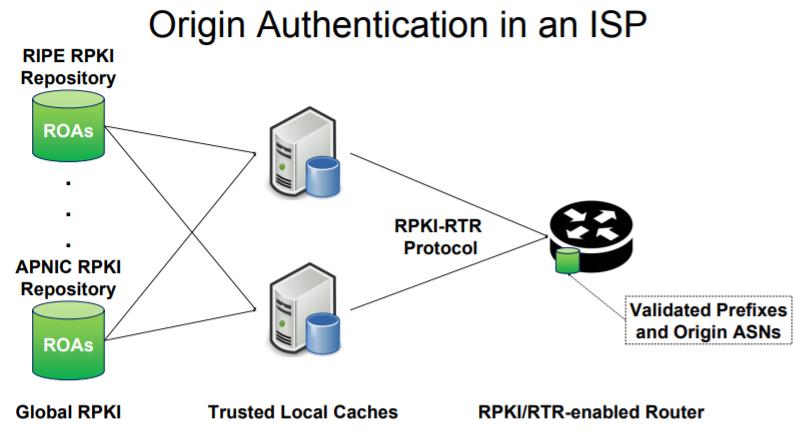
\includegraphics[scale=0.5]{images/8-origin.PNG}
	\caption{Origin authentication in an ISP.}
	\label{fig:bgp1}
\end{figure}

\textbf{Operation:} 1) Receive announcement for prefix v from AS M. 2) Check against ROAs in RPKI for prefix v. 3) Accept if valid ROA for AS M is found, else drop announcement.

\textbf{Not enough:} A malicious AS can append itself on the path with a valid ROA for certain prefix and attract (a fraction of) traffic for legitimate AS.

\paragraph{Solution 2: BGPsec}
BGPsec secures the AS-PATH attribute in BGP announcements and prevents the crafting of a valid origin by prepending ASes along with path poisoning. It's basically origin authentication $+$ cryptographic signatures. Received messages are signed to prove that a path was correctly updated (next AS is included in the signature). %TODO: more

BGPsec can validate that the AS path indicates the actual order of traversed ASes and disables modifications (adding/removing an AS). RPKI is used to verify AS key material (similar to solution 1).

BGPsec is in incremental deployment which allows for protocol downgrade attacks (if security is not prioritized when dealing with non-BGPsec BGP routers). It is challenging to figure out how to effectively prioritize security (over business relationships). Furthermore, performance is degraded since BGPsec does not allow for prefix aggregation and involves complex crypto (slower convergence).

Challenges for large-scale deployment include: different message formats, complete and accurate registries and PKI. In general, upgrading equipment is expensive, cooperation amongst many entities is required and the benefits are unclear for first-movers.

\paragraph{Extensive Monitoring}
Another approach to problem 2. BGP update messages are monitored and compared to past history. Remember which AS originates which prefix and AS-level edges / paths. Delay adoption of unfamiliar routes if possible.

This can be realised with an out-of-band detection mechanism (e.g. \textit{ARTEMIS}, \textit{Prefix Hijack Alert System}, etc.).

\paragraph{SCION}
Proposal to redesign inter-domain routing since BGP was not created with security in mind. Introduces trusted entities, enables simple security patches, etc. Other approaches include Named-Data Networking / Information-Centric Networking, Accountable Internet Protocol, Passport: Secure and Adoptable Source Authentication, etc.

\newpage

\section{Real World Network Security}

%TODO: watch lecture

Guest lecture, more just experiences with it. 
\newpage

\section{(Distributed) Denial of Service Attacks}

\paragraph{Denial of Service Attack}
Making a service or network resource unavailable to its intended / legitimate users. Typically achieved by exhausting available resources by sending an excessive amount of traffic.

To mitigate such attacks, it is common to use a combination of various mitigation techniques at different points in the network hierarchy.

First, an attack has to be detected (by comparing it to normal / human traffic patterns) and then it has to be filtered.

\paragraph{Distributed DoS Attack}
Many different sources simultaneously (often with botnets). Often used to extort companies. Harder to track and take down than a regular DoS attack and also easier to hide identity. Allows for a virtually unlimited bandwidth for flood attacks.

\paragraph{Attack Targets}
See Figure \ref{fig:ddos_target} for an overview.

\begin{figure}[h]
	\centering
	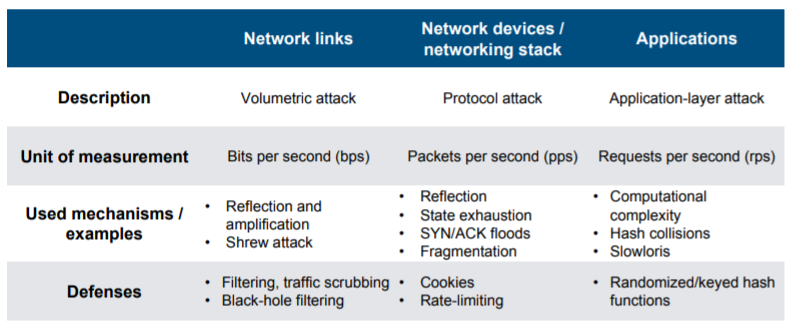
\includegraphics[scale=0.7]{images/910-targets.PNG}
	\caption{Targets of a (D)DoS attack.}
	\label{fig:ddos_target}
\end{figure}

\subsection{General DoS Attack Techniques}

\paragraph{Features Facilitating DoS Attack}
\begin{itemize}
    \item Attacker controls significantly more resources than victim.
    \item Attacker needs to expend significantly less resources than victim.
    \item Attacker can hide his identity / continually change it.
    \item Victim needs to expend a significant amount of resources before being able to assess the legitimacy of requests.
    \item Attacker can instruct / trick other entities to send traffic on their behalf.
\end{itemize}

\begin{figure}[h]
	\centering
	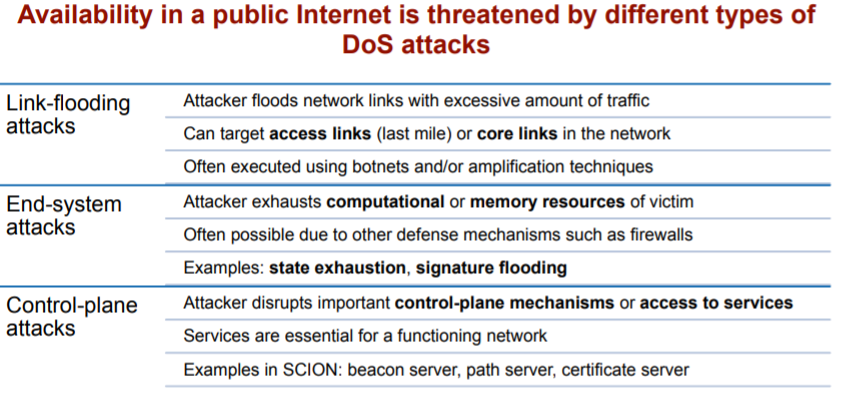
\includegraphics[scale=0.6]{images/910-attacks.PNG}
	\caption{Different kinds of DoS attacks.}
	\label{fig:attacks}
\end{figure}

\paragraph{(IoT) Botnets}
A (large) set of compromised machines (often IoT devices) connected to the Internet. They execute malicious code and can be controlled via command and control (C\&C) systems. They are often geographically distributed.

Components: command and control infrastructure to push commands to bots (often owned by attackers), zombies = devices under control of the attackers (often vulnerable hosts infected by malware) and bots - software that contains the malicious business logic.

To spread, an infected device will scan and look for open ports (e.g. sending TCP-SYN packets to randomly generated IP addresses), brute force a login, report target to controller and infect by connecting to found device and uploading malware.

IoT devices since you can have many with uniform configuration (configure-and-forget), are poorly secured (e.g. default credentials), not regularly updated (in regards to security) and often connected to the Internet without bandwidth limitations.

E.g.: Mirai botnet (mostly vulnerable webcams).

\textbf{Mitigations:} patching (automatic security updates for the device's full lifetime), credentials (not hardcoded and forced to change default passwords), monitoring (ISPs should actively monitor network for suspicious traffic).

\paragraph{Reflection and Amplification}
Need publicly accessible servers and the ability to spoof source address. Ideally, the responses caused should be (much) larger than the requests (amplification). Can be combined with a botnet consisting of master and agent nodes to exponentially grow volume.

Typical reflectors are: DNS (max. amplification 180), NTP (max. amplification 500) and Memcached (max. amplification 50'000) \footnote{Currently, NTP vulnerability is closed along with Memcached having UDP disabled.}.

An example DNS query that triggers a big response is the ANY query - it returns all DNS records of a domain (including the lengths SOA records). Nowadays, most DNS resolvers / authoritative servers refuse to respond to ANY queries or limit the response size.

\textbf{Amplification factor:} response bytes / request bytes. 

\textbf{How to:}
\begin{itemize}
    \item Choose open service as reflector (e.g. open DNS resolver).
    \item Craft a request that triggers (much) larger response.
    \item Send packet where source address is set to victim's address.
    \item Reflector sends reply to victim.
\end{itemize}

\textbf{Mitigations:} perform access control, implement response rate limiting (RRL) and ensure small amplification factors (ideally $< 1$)\footnote{WireGuard ensures that the responder's first message is smaller than the initiator's.}.

\paragraph{Address Spoofing}
Source address in an IP header can be set by the sender and in a connectionless protocol, such as UDP, a server cannot confirm the actual sender.

\textbf{Defenses:} Address filtering by ISPs (hosts should use their own addresses - would need to be globally deployed and the incentives are poor since only other ISPs profit), using connection-based protocols (such as TCP - comes with additional latency and other ways to DoS (state exhaustion)) and cryptographic source authentication (again, other attack possibilities if asymmetric crypto and requires symmetric key distribution / PKIs).

\begin{figure}[h]
	\centering
	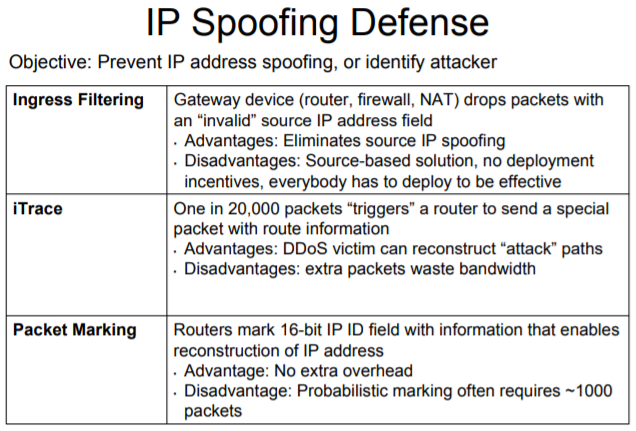
\includegraphics[scale=0.7]{images/910-ipspoof.PNG}
	\caption{IP spoofing defenses.}
	\label{fig:ipspoof}
\end{figure}

\subsection{Specific Attack Examples}

\paragraph{Volumetric: Shrew Attack}
Achieving the same effect of bandwidth-based DoS (high-rate attack traffic) with low-rate attack traffic by exploiting the TCP congestion control feature (exponential backoff if packet loss is detected).

Periodically sending short bursts to the target link / router denies the bandwidth of legitimate TCP flows at it makes TCP believe there is a long-term congestion. The bursts are most commonly send exactly when client is trying to send legitimate traffic (MITM attack in this case since the attack needs to be coordinated).

\textbf{Temporal lensing:} concentrating a low-bandwidth flood into a short, high-bandwidth pulse s.t. even a low-bandwidth attacker can perform a shrew attack. By knowing the attack path latencies, e.g. from reflector to victim, the attacker can send packets at different times to reflectors with varying path latencies s.t. overall traffic arrives at victim at the same time. With lensing, attackers can achieve peak bandwidths larger than their actual upload bandwidth. Lensing can be combined with amplification to create even larger pulses.

\paragraph{Volumetric: Coremelt}
Adversary controls botnet distributed across Internet. Bots send traffic between each other (not to victim, desired traffic). Adversary exhausts bandwidth on victim link in a per-flow fair sharing system.

\paragraph{Volumetric: Crossfire}
Adversary controls botnet distributed across Internet. Since route optimization leads to few links actually being used to target a region to rest of the Internet, adversary can contact selected servers to overload these links. Can disconnect target region from remainder of Internet.

\paragraph{Protocol: DNS Flooding / NXDOMAIN Attack}
Overwhelm the victim's authoritative name servers by querying many non-existent subdomains of victim domain. The DNS resolvers query all authoritative name servers in turn and thus a name server will not reply to legitimate requests. The more attackers and resolvers the better.

\paragraph{Protocol: Session State Exhaustion}
Two-way communication channels are identified with unique session numbers (= session state). Numbers are known at a server to match subsequent requests to right session. By exhausting the session state table of the server, it can no longer accept new connections, existing connections are dropped and maybe the server / service even crashes.

\textbf{Generic mitigations:} Encode state in a unique but determined way that allows server to validate state in client reply. No state at server is needed (other than salt). Ensure the encoding cannot be tampered (use crypto-hashes, unique data known to server only and changes over time, etc.), e.g. $B =$ Hash(salt, $A$).

\textbf{SYN flood attack:} TCP three-way handshake first message is client sending a SYN packet with a random sequence number $A$ and server keeps $A+1$ and $B$ (random seq. number of server SYN+ACK). With spoofed source addresses, a server can be flooded with SYN messages and the state table will eventually overflow.

\textbf{SYN flood attack mitigation:} SYN cookies - no state tables needed if initial TCP sequence number is particularly chosen (e.g. $B = F(\text{time, IP address, port, ...})$. Apply $F$ after ACK of client to validate and establish connection.

\paragraph{Application-Layer: Algorithmic Complexity}
Induce the worst-case behavior in a vulnerable algorithm. The larger the difference between worst and average case, the more vulnerable it is. See Figure \ref{fig:complex} for a comparison.

\begin{figure}[h]
	\centering
	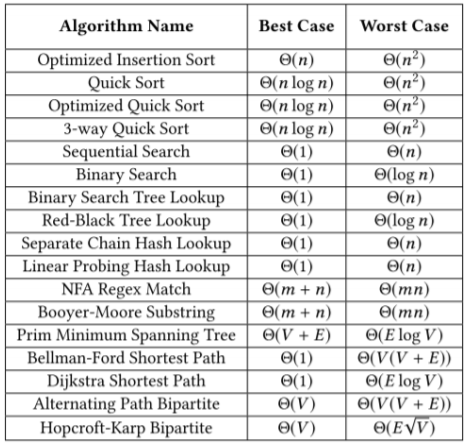
\includegraphics[scale=0.7]{images/910-complex.PNG}
	\caption{Comparison of best and worst case complexities.}
	\label{fig:complex}
\end{figure}

\textbf{Hash table lookup collisions:} collisions are common due to small size. Resolutions include chaining, open addressing, etc. An attacker can intentionally pick a bad input sequence that causes worst-case hash table collisions. Countermeasures include universal hashing (guaranteed zero to little collisions for any input), hash randomization (hard to find bad input), etc. %TODO: more?

\textbf{Regular Expression DoS (ReDoS):} provide a regular expression that takes a very long time to evaluate (matching). Most regex implementations have exponential time worst case complexity - meaning that the time taken can grow exponentially in relation to input size.

\paragraph{Application-Layer: Slowloris}
A single machine can take down another machine's web server with minimal bandwidth by:
\begin{itemize}
    \item Keeping many connections to target web server open and holding them open as long as possible.
    \item Opening connections and sending partial requests.
    \item Periodically sending subsequent HTTP headers adding to the request but never completing it.
\end{itemize}
Affected servers will keep these connections open, filling their maximum concurrent connection pool and eventually denying additional ones. 

\textbf{Mitigations:} increase max. possible connections to server, limiting connections from single IP address source, require minimum transfer speed per connection, restrict length of time client is allowed to stay connected. Or: set up reverse proxies, firewalls, load balancers or content switches.

\subsection{Countermeasures}

\begin{itemize}
    \item \textbf{Ingress Filtering:} Remove packets with illegitimate source IPs.
    \item \textbf{Computational Puzzles:} Slows down attacks, achieves per-computation fairness.
    \item \textbf{Cloud- or ISP-based Filtering:} Delegates defense to cloud / ISP.
    \item \textbf{Network Capabilities:} Allows victims to block unwanted traffic closer to the source.
    \item \textbf{IP Traceback:} Reveals real source IP of packets.
\end{itemize}

\paragraph{Guarantee Little Downtime}
\begin{itemize}
    \item \textbf{Redundancy:} No single point of failure, $N+2$ systems running under normal operation (if two systems fail, service still available), $> 2$ geographically diverse connections / independent Internet connections.
    \item \textbf{Monitoring and Rapid Detection / Automatic Failover and Eviction:} Long term monitoring to assess periodicity and peak periods / loads. Over provision such that resources cover majority of extreme peak loads (average can be misleading).
    \item \textbf{Failure Resiliency:} System can tolerate various temporary component failures and gracefully degrades upon too many.
\end{itemize}

\paragraph{Cloud-Based DDoS Mitigation Service}
Traffic can be redirected to a cloud provider for filtering or content delivery by changing BGP / DNS (scrubbing / rerouting). Some provide CDN service to serve requests from many locations.

Can be easily bypassed if the victim's IP is exposed since most clouds use DNS (BGP-based is harder to bypass). Also prone to privacy violation. High cost and requires continuous subscription.

\paragraph{In-Network- / ISP-Based DDoS Mitigation Service}
ISP redirects traffic to high-capacity scrubbing center and sends back filtered traffic to destination (always or on demand). Scrubbing center uses deep packet inspection (DPI) and connection patterns to filter malicious traffic.

\paragraph{Remotely Triggered Black Hole (RTBH) Filtering}
Can be used to mitigate volumetric attacks. Install rules to drop traffic based on source or destination addresses in border routers of an AS (= black hole). Can be achieved through BGP updates (most likely triggered by manual intervention).



\subsection{SCION}

One way to completely redesign the internet. Achieving global communication guarantees on the public internet (high security, formal verification from the start). High efficiency due to path-aware networking - sender knows the path and can select among options - and multi-path communication (= path optimization and load balancing). Additional principles include: 

\begin{itemize}
    \item Stateless packet forwarding (routers keep almost no state, no risk for inconsistent forwarding state)
    \item Instant convergence routing (all paths are instantaneously usable)
    \item Sovereignty and transparency for trust roots
    \item Per-packet authentication and verification possible on routers
    \item Formal verification of protocols and code
    \item Immune against routing attacks (e.g. BGP prefix hijacking)
\end{itemize}

\begin{figure}[h]
	\centering
	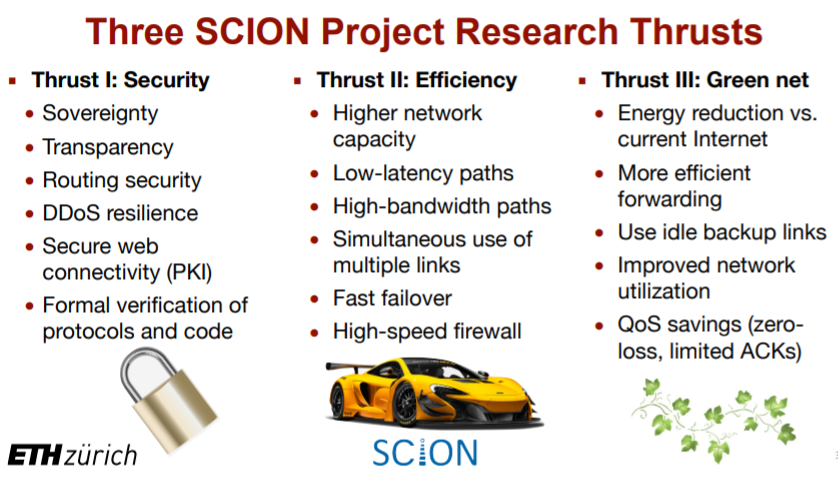
\includegraphics[scale=0.7]{images/910-why.PNG}
	\caption{SCION goals / motivation.}
	\label{fig:why}
\end{figure}

\subsubsection{SCION Overview}

\paragraph{Isolation Domain (ISD)}
A grouping of autonomous systems. An ISD has a core consisting of ASes that manage it and provide global connectivity (upstream = reach core). Each ISD has a root of trust governing it (trust root configuration, TRC) and can thus function autonomously without external trust.

\paragraph{Control Plane}
Responsible for the routing mechanisms. In SCION, the control plane constructs (path exploration) and disseminates (upon sender request) path segments. Each AS contains border routers, beacon servers and path servers. The control plane is also responsible for the dissemination and renewal of certificates needed to verify segments.

\textbf{Intra-ISD Path Exploration:} Done with beaconing. The core ASes initiate path-segment construction beacons (PCBs) which are flooded throughout the entire ISD - downstream ASes learn how to reach core ASes through the paths that the PCBs have taken (on the way down, each AS that sees the PCB appends itself as a next hop, additional to a MAC and its signature).

\textbf{Inter-ISD Path Exploration:} Same concept, just a lot denser than in the intra case. PCBs are distributed only among core ASes to create core-path segments.

\textbf{Path Server Infrastructure:} Path servers offer a lookup service (similar to DNS) to find down-path, up-path and core-path segments. The core ASes of each ISD operate the core-path and down-path server infrastructure (consistent and replicated) - selected path segments are chosen, stored and announced globally. Each non-core AS runs local path servers that serve selected up-path segments to local clients (no global announcements) along with resolving and caching responses of remote AS lookups.

In total, a host fetches the local up-path segments, global down-path segments and core-path segments if needed (to connect up- and down-path segments) by contacting its local path server with (ISD, AS) which might contact more path servers if info is not cached - this created an end-to-end path (which might be shorter than all segments combined - see yellow paths in Figure \ref{fig:paths}).

\begin{figure}[h]
	\centering
	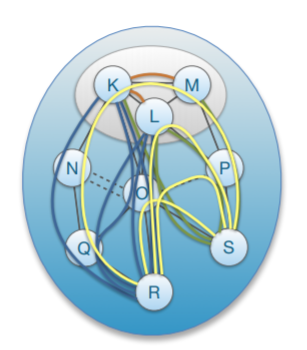
\includegraphics[scale=0.7]{images/910-path.PNG}
	\caption{Possible end-to-end paths from AS R to AS S (in yellow).}
	\label{fig:paths}
\end{figure}

\textbf{Path Combinations:} Not all path combinations are feasible due to security reasons. See Figure \ref{fig:combis} for all possible combinations.

\begin{figure}[h]
	\centering
	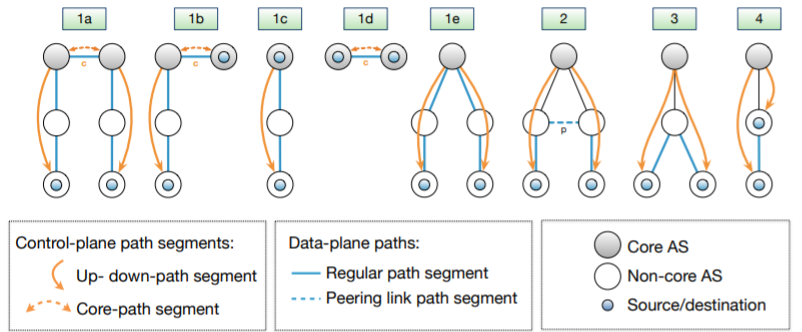
\includegraphics[scale=0.8]{images/910-combis.PNG}
	\caption{All possible ways to combine path segments.}
	\label{fig:combis}
\end{figure}

\paragraph{Data Plane}
Responsible for the actual packet forwarding. Path segments are combined to form a path. Segments (plus some metadata like geographical location or link latency) are included in the packet header (encrypted), therefore a sender knows exactly which ASes are traversed. A router only verifies the authenticity of the information (two AES operations replace longest-prefix match).


\paragraph{SCION Drawbacks}

\begin{itemize}
    \item Initial latency inflation to obtain paths during lookup (amortized by caching and path reuse since most destinations are reused).
    \item Bandwidth overhead due to paths in the packet headers - around 80 additional bytes (but enables path control and a simpler data plane).
    \item Increased complexity in key management due to new certificates like TRC certificates (necessary for a high security design).
    \item Initial set-up cost due to training network operators and installing new infrastructure (methods exist to facilitate deployment and new properties become possible with it).
\end{itemize}

\paragraph{SCION Deployment}
Since the AS infrastructure inside an ISP is being reused, there is not a lot of change necessary in the internal network infrastructure. We just need to set up core routers at the borders of an ISP (peering with other SCION-enabled networks and collect customer accesses). For end domains, we just need a SCION IP gateway (SIG) that enables seamless integration of SCION capabilities in end-domain networks. SIGs are then connected to SCION (border) routers. No upgrades of end hosts / applications are needed, it's just an additional packet header.

Incremental deployment is possible. Important to not rely on BGP for inter-domain operation s.t. we don't inherit its vulnerabilities. For local communication, intra-domain network architecture can be reused (intra-domain routing).


\subsubsection{SCION Security Insights}

\paragraph{Global Communication Guarantees}
Especially in the presence of adversaries. Goal: if a (routing policy compliant) path of good ASes exist, a sender can find, use and achieve minimum bandwidth guaranteed on that path. Challenges include: network routing instabilities / misconfigurations and DoS attacks are various levels (control and data plance, end hosts, etc.).

\textbf{Stable Forwarding and Multi-Path:} for the first challenge, these two concepts are necessary. Single-path forwarding cannot achieve strong availability guarantees (convergence, equipment failure, packet loss - path available / connectivity but shitty and needs manual intervention, etc.). With stable forwarding we have packet-carried forwarding state that protects forwarding from routing instabilities. With multi-path, we ensure the presence of several paths and as long as one works, end-to-end connectivity is assured. Overhead is low with the path segment combination method (instead of full paths). But, secure routing is insufficient in the case of outages caused by bottleneck links or continuing announcement of failed / congested routes since announcements in these cases are still legitimate.

\textbf{DoS Attacks:} SCION has several components that guarantee strong security and high availability (see Figure \ref{fig:secure}).

\begin{figure}[h]
	\centering
	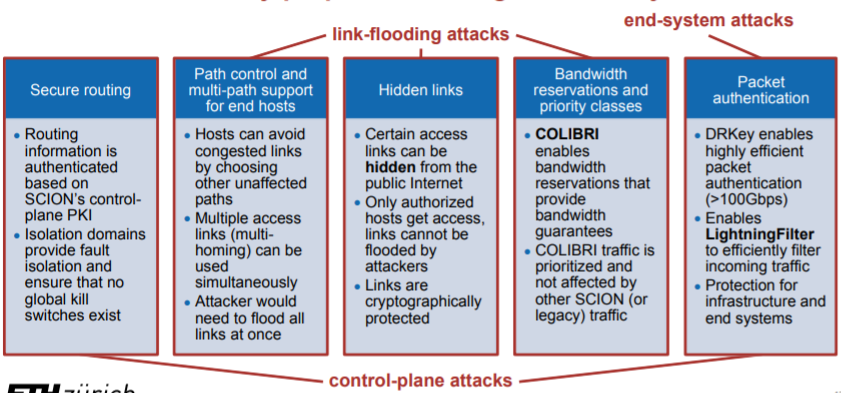
\includegraphics[scale=0.8]{images/910-secure.PNG}
	\caption{SCION protecting against DoS type attacks.}
	\label{fig:secure}
\end{figure}

\paragraph{High-Speed Packet Processing}
If you do it right, cryptographic operations can be performed on a per-packet basis. E.g. with a 400 Gbps link, a 64-byte packet arrives every 1.3ns. Symmetric crypto enables high-speed processing through parallel processing and pipelining - e.g. taking only around 100$\mu$s per signature (compared to a DRAM memory lookup that takes around 70ns). Not possible with asymmetric crypto. %TODO more here?

SCION offers a global framework for authentication and key establishment for secure network operations. DRKey = dynamically recreatable keys - creating crypto keys on the fly (within 20ns). With DRKey and EPIC, per-packet source authentication in software possible under 100ns. Control-plane PKI means that every AS has a public-key certificate that enables AS authentication and for each ISD to operate in a sovereign manner.

\textbf{DRKey:} use a per-AS secret value to derive keys with an efficient pseudo-random function (AES operation). With the secret value, a key created for another AS can be derived (fast) but without it (other AS) the key has to be fetched by contacting a local key server.

\textbf{Key Server Infrastructure:} each AS has a key server building the backbone of the key hierarchy. Servers are responsible for key exchange, management and local key establishment. After establishing AS-level keys, symmetric keys for end hosts can be provided and used to provide source authenticity of packets (without a costly key exchange). Each host is required to contact their local key server. See notes for a better explanation. %TODO example SCMP (exercise 13 as well), below

\textbf{LightningFilter:} SCION firewall that authenticates packets at very low overhead (no FP/FN, no heuristics). Sender locally fetches remote LightningFilter's DRKey and the filter then authenticates packets by deriving the DRKey. Normal to combine it with normal firewall (LF at border and firewall closer to destination). Also allows for history-based filtering by keeping track of rate of key requests of AS (and blocks if they overshoot). And duplicate suppression with bloom filters.

\textbf{EPIC: Every Packet Is Checked:} per-packet source authentication by every router and destination - possible with DRKey and a per-packet unique hop field (no duplication possible). Assumes global time synchronization. Same as in LF, source needs to first fetch all the keys to compute per-hop fields. Prevents malicious router replays / amplification and MAC bruteforce. %TODO hm, esp hop field thingy

%TODO comparisons with BGP / results at end of lecture

\paragraph{COLIBRI}
Provides practical and scalable global QoS. Stable paths that ensure reservations are not affected by routing changes. Multi-path system to search for paths with sufficient bandwidth. No per-flow state on routers (enables scalability) - possible with DRKey (per-packet source authentication), probabilistic large flow detection to detect overuse, per-flow stateful control-plane (server infra). Per-neighbor fairness (admission decision, ISP configs). %TODO ?? reservation?

\textbf{Admission Algo with Per-Neighbor Fairness:} instead of per-flow fairness (normal Internet), we have per-neighbor fairness. Each AS defines N2N minimum bandwidth guarantees (that can be computed for any path). Algo guarantees that no set of ASes can reserve a disproportionate amoung of bandwidth through any link. %TODO: example, how to compute??

\paragraph{Bandwidth Reservation}
Simplifies transport layer due to no need for sophisticated congestion control (simply use constant bitrate - good for streaming traffic). Low loss rate - low amount of ACKs. Enforce fairness at level of admissions. Traffic engineering.

%TODO scion vs. ip and bgp (exercise 13 and lecture)



\newpage

\section{Firewall Intrusion Detection and Evasion}

\subsection{Overview}

\paragraph{Firewall}
A system protecting or separating a trusted network from an untrusted one. It either permits, denies or proxies data through a network with different levels of trust. = Access control policy between two networks.

This is not enough. Many ports need to be kept open for legitimate applications to run. Evolution messes with legacy firewall technology (P2P. instant messaging, Web 2.0 - multiple functions for single-function port, etc.).

\textbf{Network firewall:} Software appliance running on specific hardware or as a virtual instance. Filters traffic between two or more networks. Protects different network segments.

\textbf{Host firewall:} Layer of software on a host that controls traffic going in and out of a single machine. Protects single host.

\textbf{Stateless firewall:} Examine a packet at the network layer and base decision on packet header information. Application independent and good performance / scalability, but no context.

\textbf{Stateful firewall:} Also keep track of state of network connections and base decision on packet header and session state. More powerful rules are possible but state can be inconsistent / nonexistent (UDP) and explode ((D)DoS).

\paragraph{Filtering Rules}
\begin{itemize}
    \item \textbf{Ingress:} Incoming traffic, low to high security network.
    \item \textbf{Egress:} Outgoing traffic, high to low security network.
    \item \textbf{Default:} Define what to do if no rule matches (accept / reject).
    \item \textbf{Deny Access:} Either silently drop or reject (\textit{ICMP Destination Unreachable}) packet.
\end{itemize}

\paragraph{Next Generation Firewall (NGFW)}
Performs deep packet (payload) inspection and takes application and protocol state into account (on top of typical firewall functions). Allows for powerful rules and application / protocol awareness. Cons: needs to support many application protocols, impacts performance / scalability, deals with inconsistent state (host vs. firewall), etc. %TODO: more? examples?

\paragraph{Web Application Firewall (WAF)}
Protects web-based applications from malicious requests by filtering based on requests / signatures (SQL injection, cross-site scripting, buffer overflow, checking number of form parameters, etc.). Allows for static or dynamic black- / whitelisting. Con: false positive problem.

WAFs are often implemented as a reverse proxy (client outside of internal network) to protect public facing web applications.

\paragraph{Deployment Challenges}
How to protect a large number of hosts / endpoints / network segments.

\begin{itemize}
    \item \textbf{Complexity:} Rules can be complex, thousands of rules per firewall are common, detection between channels is out of sync (mail vs. net vs. proxy).
    \item \textbf{Management:} How to change / remove rules? Who has the permission? What tools?
    \item \textbf{Incentives:} Infrastructure team is paid for providing connectivity and blamed for disruptions and security team is paid to protect and disrupt connectivity...
\end{itemize}

\subsection{Firewall Attack Methods}

\paragraph{IP Source Spoofing}
Spoofing the source IP address. Works for stateless protocols (e.g. UDP, ineffective for TCP).

\paragraph{Artificial Fragmentation}
A fragmented packet might pass a firewall if it's not able to properly reassemble it (e.g. because they're out of sequence). For example, the port number is only in the first fragment. Also works by splitting the attack into multiple packets or overlapping the individual fragments.

\paragraph{Denial of Service}
Firewall state explosion. Need to define a good fallback policy.

\paragraph{Tunneling / Covert Channels}
Creating a capability to transfer information between processes that are not supposed to communicate. For example, putting data in ICMP ping packets or using DNS requests as a channel. Furthermore, attacks can also be performed through a VPN tunnel.

\paragraph{Payload Encodings}
Use different encodings allowed on the protocol / application in use and addition of noise to confuse detection. Different encoding and obfuscation schemes can be combined with noise insertion in millions of ways and encodings are not necessarily unique. Furthermore, undefined or border cases are very effective for detection evasion. There might also be different implementations of decoding on target application vs. detection engine decoding.

%TODO better examples?

E.g.: URL encodings (\% encoding, path character tranformations) or HTML obfuscations (UTF-7 / UTF-16 / UTF-32 character set encoding, chunked encodings, different compression schemas, Base64 encoding, etc.).

\begin{figure}[h]
	\centering
	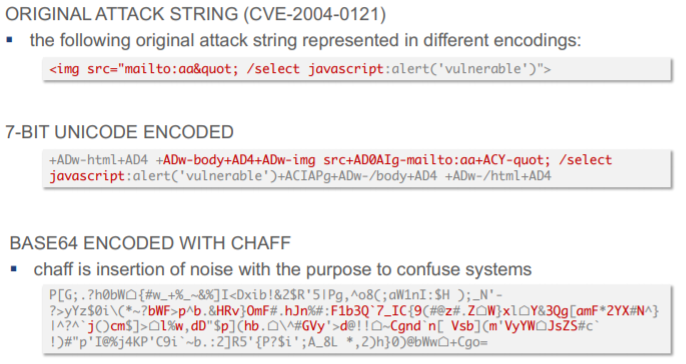
\includegraphics[scale=0.8]{images/911-encodings.PNG}
	\caption{Attack string in different encodings.}
	\label{fig:encoding}
\end{figure}

\paragraph{Firewall Vulnerabilities}
There are several vulnerabilities found in firewall software from security vendors. Firewalls are complex! See examples in Figure \ref{fig:vulnerable}. 

\begin{figure}[h]
	\centering
	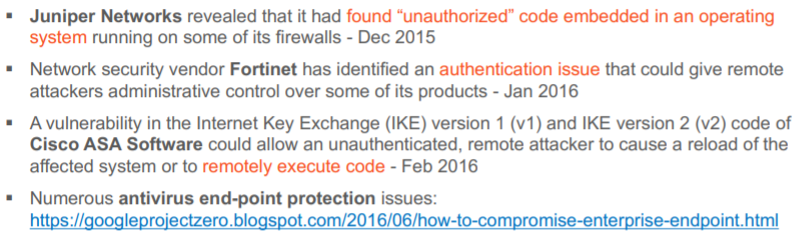
\includegraphics[scale=0.8]{images/911-vulnerable.PNG}
	\caption{Some vulnerabilities found in commercial firewalls.}
	\label{fig:vulnerable}
\end{figure}

\subsection{Intrusion Detection Methods}

\paragraph{Key Features of Intrusion / Attack Detection}
\begin{itemize}
    \item \textbf{Reactive:} System can only detect already known attacks.
    \item \textbf{Proactive:} System can detect known and new, yet unknown attacks.
    \item \textbf{Deterministic:} System always performs the same given the same input. Reason for alert is known.
    \item \textbf{Non-Deterministic:} Detection is fuzzy (heuristics, ML, sandboxing, etc.) and depends on state. Reason for alert is typically not known.
\end{itemize}

\paragraph{Detection Techniques}
See basic detection approaches in Figure \ref{fig:techniques}.

\begin{figure}[h]
	\centering
	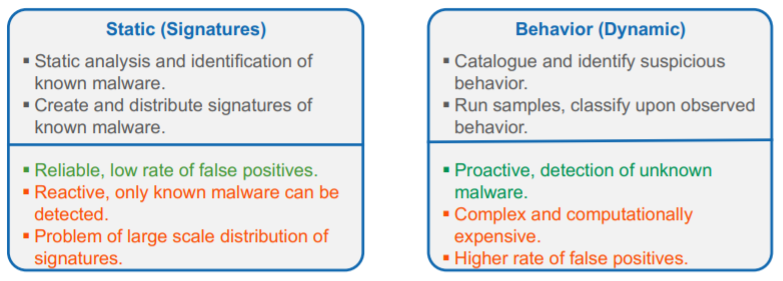
\includegraphics[scale=0.8]{images/911-techniques.PNG}
	\caption{Basic approaches to intrusion detection.}
	\label{fig:techniques}
\end{figure}

Key features include:
\begin{itemize}
    \item \textbf{Protocol Analysis:} Analysis and decoding of protocols. Reassembly and normalization of traffic.
    \item \textbf{Signatures:} Compare attributes of observables to black- / whitelists or to patterns of known attacks / exploits / malware. A signature can be simple groups of checksums / byte arrays or complex hundred lines of code.
    \item \textbf{Sandboxing / Behavior:} Suspicious file is executed within a virtual environment. Specific actions are categorized and labeled as good / bad.
    \item \textbf{Machine Learning:} Recognize complex patterns and make decisions based on data / assumptions formed from previous data. Learn (good vs. bad), extract features, train and test.
    \item \textbf{AI:} not just learning how to solve a specific task very well (ML) but actually learning how to improve itself to solve new previously unknown tasks. Goal: increase chance of success, not accuracy.
\end{itemize}

Signature based approaches will stay and be accompanied by more sophisticated unsupervised ML approaches.

\paragraph{Signature Based Detection}
Core concepts still lie at the heart of all modern detection systems and will continue to be integral for the foreseeable future. Reactive and deterministic. Progression / Sophistication of such systems depend on human signature writers. Bad with mutations / polymorphism. Characteristics:

\begin{itemize}
    \item Able to promptly identify and label a threat.
    \item Different signature systems are used together for more accuracy.
    \item Unique signatures or signature artifacts are created for new threats.
    \item Signature databases / online lookups are frequently updates.
\end{itemize}

Indicators of Compromise (IoC) similar, not a full signature (mostly IPs or file hashes). E.g. Yara Rule.


\textbf{One-Dimensional:} common in all systems, fastest and most efficient way of categorizing a data artifact. Simply a boolean output (good / bad). Doesn't need many resources, is fast and has a low number of false positives but is reactive, needs frequent updates to signatures and uses humans.

\textbf{Two-Dimensional:} regular expression functions and string matching, fundamental for anti-malware / IDS / DLP systems, easily capable of identifying previously known exploits and host enumeration techniques. Low / medium resource requirements, more flexibility with patterns and low false positive rate. Cons: same as above.

\textbf{Multi-Dimensional:} instead of triggering on a single signature, a multi-dimensional signature was created, can label actions as suspicious or bad (sandboxing / network behavioral monitoring). Classify and label threat after a certain threshold of good or bad activities is met. Is partially proactive and more efficient / effective than above approaches.

\paragraph{Sandboxing Based Detection}
Basically running malware in a detonation chamber by examining / monitoring runtime behaviour of a sample and comparing behavior against a list / rules previously developed in a lab or via machine learning (behavior classification - no humans!). Is proactive and mostly deterministic. 
Doesn't require updates to signatures. Cons: resource intensive, high latency and difficult to scale.

\paragraph{Limitations of Intrusion Detection}
\begin{itemize}
    \item Unable to inspect encrypted traffic.
    \item High number of false positives.
    \item Packet capturing and analysis at high link speed (tens of Gbits/s).
    \item Minimize latency introduced by inspection engine.
    \item Application level attacks (JavaScript, etc.).
    \item Policy / signature management.
\end{itemize}

\paragraph{Accuracy vs. Precision}
For decision making (block/pass) the consistency of accuracy is most important. Accurate detection is very challenging (balance zero FN and zero FP). 

%TODO see examples p. 59!! Sensitivity vs. specificity stuff

\textbf{Accuracy:} how close is the measured value to target value (bias).

\textbf{Precision:} Values of repeated measurements are clustered and have little scatter. Can be far away from target value (variance).

\begin{figure}[h]
	\centering
	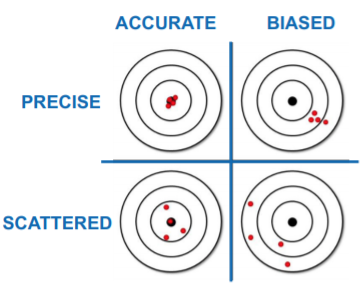
\includegraphics[scale=0.6]{images/911-accprec.PNG}
	\caption{Accuracy vs. precision.}
	\label{fig:accprec}
\end{figure}

\begin{figure}[h]
	\centering
	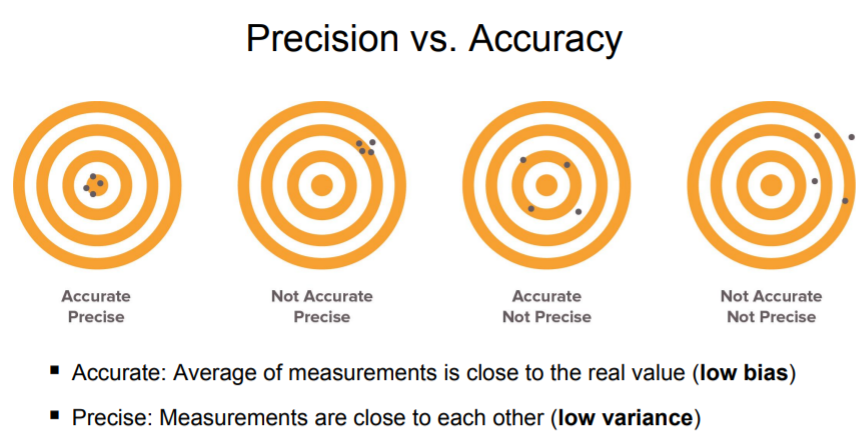
\includegraphics[scale=0.6]{images/911-another.PNG}
	\caption{Another accuracy vs. precision.}
	\label{fig:another}
\end{figure}

\begin{figure}[h]
	\centering
	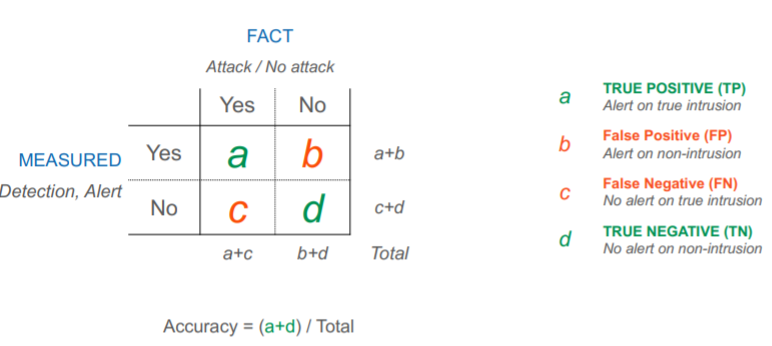
\includegraphics[scale=0.8]{images/911-positives.PNG}
	\caption{Accuracy and type of measurements.}
	\label{fig:positives}
\end{figure}

\paragraph{Sensitivity vs. Specificity}
Sensitivity measures the proportion of positives that are correctly identified (TP / all positives resp. FN + TP). Specificity measures the proportion of negatives that are correctly identified (TN / all negatives resp. FP + TN).

\paragraph{Detection Performance}
\begin{itemize}
    \item Accurate detection is very challenging when rate of attacks is very low.
    \item Different detection techniques achieve different sensitivity and specificity.
    \item Use a combination of diverse tests to increase precision.
    \item Context is important (host vs. network based detection).
\end{itemize}

\begin{figure}[h]
	\centering
	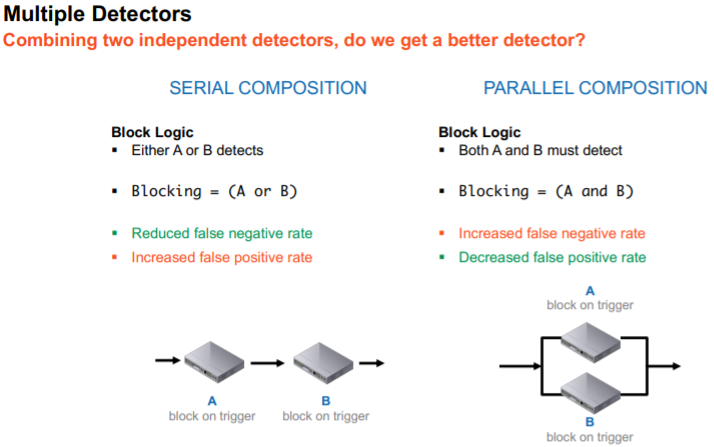
\includegraphics[scale=0.6]{images/911-combine.PNG}
	\caption{Multiple detectors.}
	\label{fig:detect}
\end{figure}



\subsection{Layered Security - Filtering and Protection}

% TODO?


\subsection{Detection Evasion by Design}

\begin{figure}[h]
	\centering
	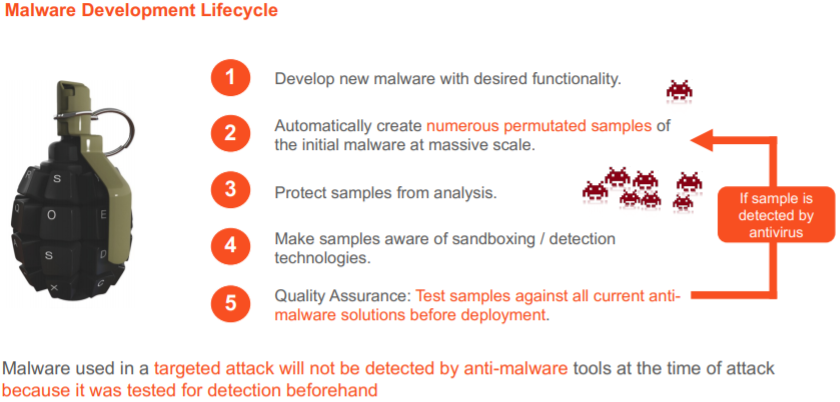
\includegraphics[scale=0.6]{images/911-malware.PNG}
	\caption{Malware development life cycle.}
	\label{fig:malware}
\end{figure}

\paragraph{Step 1: Create Initial Malware}
Create malware core functionality, such as key logger, web-injection, attacks, spreading, communication, etc. by hiring a coder, buying / stealing it or do it yourself.

\paragraph{Step 2: Crypter and Serial Variants}
Encrypt it s.t. signature detection systems and static analysis processes are ineffective. Use different keys to create serial variants / permutations. Encrypt contents of malware executable. Upon execution, only decrypt sections of code on the victim's computer.

\paragraph{Step 3 and 4: Protection Against Debugging}
Use protector technology that detects the use of debuggers or virtualization techniques. If seen, a malware can do different operations (hiding malicious intention or trigger exploitation of virtual environment). %TODO examples

\textbf{Polymorphism techniques:} How to mutate code while keeping the original algorithm intact. Done by manipulating structure of source code of malware by reordering and replacing common programmatic routines. Swapping of equivalent code constructs, changing order of code (registers, instructions, function definitions), inserting noise (redundant code, non-occurring exceptions, functions that are not called), compiler modulation (different compilers can result in different binary code output), etc.

\paragraph{Step 5: Quality Assurance}
Pass malware through many commercial antivirus products (automated). Only use services that do not submit malware samples to vendor! %TODO examples?

%TODO: detection example p.49, watch recording



\newpage

\section{Malware Analysis and Prevention}

\subsection{Threat Analysis}

\paragraph{What to do with a Potential Threat} 
After finding out what to analyze, do automated testing to get a first impression - we may already know it. One can use internal sandboxes or use scanners. However, many malware samples try to prevent automated analysis (can detect a VM). Use a hex editor to find out if it's a portable executable (e.g. .exe) file. Such files have a distinct and well-defined structure.

Analysis generates a lot of metadata that one can further analyze and put into a database for clustering (e.g. does a website host a lot of malicious URLs?).

\paragraph{Blackboxing (Dynamic Analysis)}
Executing a sample on a dedicated system (virtual or real) to see what it does (not interested in how, we just wanna know what kind of malware it is). Monitor all system API calls, analyze logged information, dump decrypted content from memory (if malware is originally encrypted), etc.

Blackboxing can't tell you everything! Use Whiteboxing as well.

\paragraph{Whiteboxing (Static Analysis)}
Actually analyzing and reading the code by using a debugger or a disassembler. Can be helpful to find hidden functions (e.g. just doing malicious things on a specific day/condition, etc.).

\subsection{Prevention Methods}
A detection rate without knowing the false positive rate is useless. You could just classify everything as malicious to catch all malware (high false positive rate).

Also, see Firewall chapter.
%TODO: combine

\paragraph{Main Types}
\begin{itemize}
    \item \textbf{Pattern Matching:} signatures, static ML, data loss prevention, etc. - what is it?
    \item \textbf{Analysing Behavior:} anomaly detection, post-execution ML, web application firewall, etc. - what does it do?
    \item \textbf{Prevent Unwanted Access/Changes:} hardening, firewall, app isolation, etc.
\end{itemize}

\paragraph{Some Other Protection Concepts}

%TODO ???

\begin{itemize}
    \item \textbf{Deception:} honeypot an attacker.
    \item \textbf{User Entity Behavior Analysis:} zero trust.
    \item \textbf{Endpoint Detect and Response (EDR / XDR):} 
    \item \textbf{Network-Based Detection and ISP:} anomaly detection in network, etc.
\end{itemize}
\newpage

\section{Internet of Things}

\paragraph{Safety vs. Security}
Safety is the protection against random, unwanted incidents - resulting from coincidences or driven by the environment (which does not adapt to bypass safety measures). Security is the protection against intended incidents - resulting from a deliberate planned act and driven by targeted attacker.

%TODO: intro slides? examples, generally how important?

\begin{figure}[h]
	\centering
	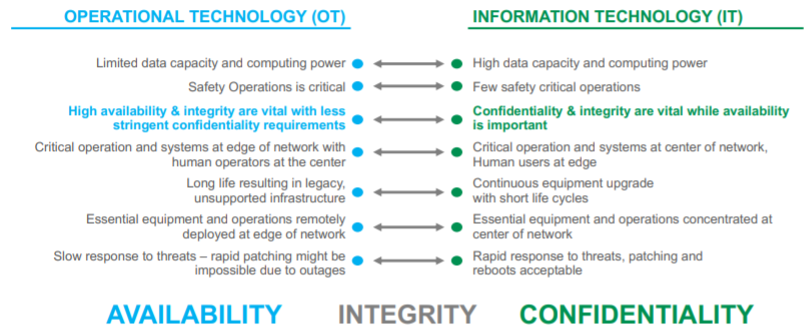
\includegraphics[scale=0.8]{images/913-otvsit.PNG}
	\caption{Key differences between operational and information technology.}
	\label{fig:ot}
\end{figure}

\paragraph{Attack Surface}
IoT connects innumerable everyday devices and systems. Devices can have insecure software / vulnerabilities and insecure defaults, cheap components, be lacking of an update mechanism. Furthermore, since they're replicated, finding a fault in one can give access to all (no unique identity). Backend service is the central control and can be attacked in regards to data (breaches, privacy, etc.). Both ends are connected with by an insecure communication channel (weak or no crypto, lack of authentication, etc.). Now, closed systems are opened up to remote access and control!

IoT devices are perceived to have very low risk in comparison to a computer. An attacker can exploit this risk perception (easy targets).

IoT devices are mainly designed to have high availability with safety but no security. They need continued security maintenance. Also, certification timeline is often outpaced by cyber security (patches make a certification unusable).

\begin{figure}[h]
	\centering
	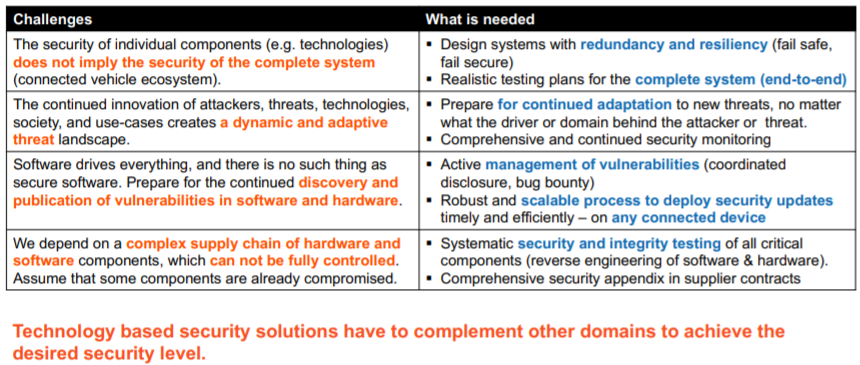
\includegraphics[scale=0.8]{images/913-conclusion.PNG}
	\caption{Summary of IoT lecture.}
	\label{fig:conclusion}
\end{figure}
\newpage

\section{Supply Chain Security}

Not covered in lecture.
\newpage

\section{Domain Name System Security}


\paragraph{DNS}
Main function is to provide a mapping of names to resources of several types (e.g. resolving a domain name to an IP address) in a hierarchical and decentralized fashion. It is a globally distributed, loosely coupled, scalable, reliable and dynamic database. Data is maintained locally and retrieved globally.

\begin{figure}[h]
	\centering
	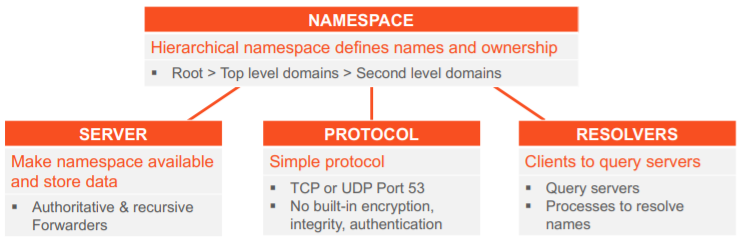
\includegraphics[scale=0.8]{images/915-dns.PNG}
	\caption{DNS key components.}
	\label{fig:dns}
\end{figure}

\paragraph{DNS Security is Critical}
Manipulating the DNS mapping allows an attacker to redirect connections, perform MITM / impersonation attacks and to launch DoS attacks. For an attacker, a DNS is a freely available distributed storage system or can be used to setup services that are hard to hunt / shut down (e.g. botnets, fast- and domain flux).

\paragraph{DNS Namespace}
A distributed global lookup mechanism for translating names into other objects organized in a hierarchy (see Figure \ref{fig:namespace}). Authoritative name servers are responsible for mapping domain names to actual Internet resources for each domain (configured by an admin). For each domain, one can define DNS zones that contain a number of distinct sub-level domains (= leaf-nodes).

\begin{figure}[h]
	\centering
	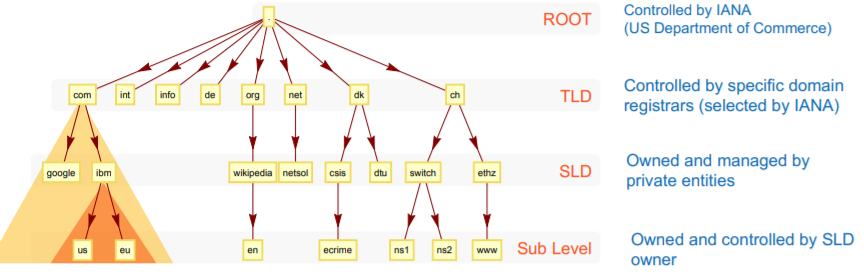
\includegraphics[scale=0.8]{images/915-namespace.PNG}
	\caption{Hierarchical DNS namespace.}
	\label{fig:namespace}
\end{figure}

\paragraph{DNS Resolution}
When a client makes a DNS request for a specific domain, it can go through many levels of delegations as depicted in Figure \ref{fig:resolution}.

\begin{figure}[h]
	\centering
	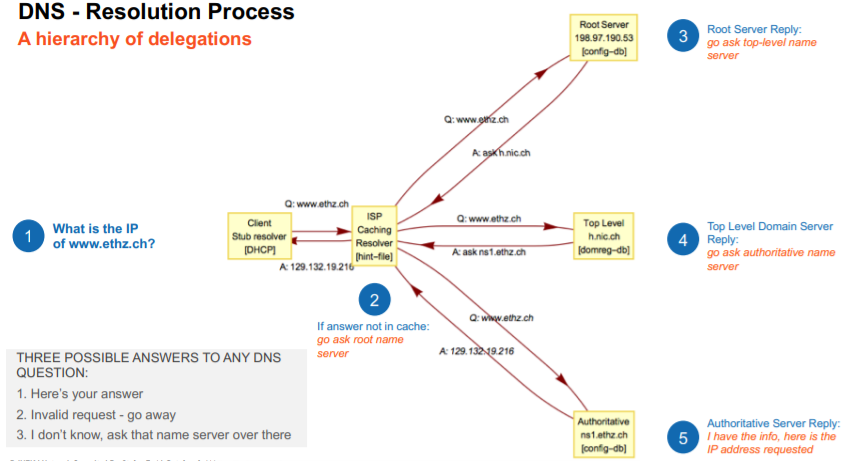
\includegraphics[scale=0.8]{images/915-resolution.PNG}
	\caption{DNS resolution process.}
	\label{fig:resolution}
\end{figure}

Resources\footnote{If a domain request couldn't be resolved in the past, it is cached with an \textit{NXDOMAIN} entry, meaning nonexistent domain.} can be cached at many points during the hierarchical query process. Cache expiration is controlled by the TTL attribute of an entry.

Requests can be resolved recursively, non-recursively or iteratively (or a combination).

\textbf{Recursive:} DNS resolver queries single DNS server which may in turn query other DNS servers. The resolver answers a query completely by querying others as needed.

\textbf{Non-recursive:} DNS resolver queries a DNS server that is either authoritative or provides a partial result.

\textbf{Iterative:} DNS resolver queries a chain of one or more DNS servers. Each server refers client to the next server on the chain until the current one can fully respond.

\paragraph{DNS Key Protocol Features}
To protect against forged responses, the first two bytes in a message form a transaction ID (\textit{txid}) that must be the same in query and response and introduces 16 bits of entropy ($2^{16}$) - it is set randomly by the client. DNS messages can either use TCP or UDP (port 53).

\textbf{Security:} If the \textit{txid} does not match, client drops response. Furthermore, client can choose a random source port (16 bits of entropy). There is no confidentiality, integrity verification nor authenticity.

\paragraph{DNS Resource Record (RR) Types}
RRs define data types in DNS. Each record has a type (name and number), a TTL, a class and type-specific data. See Figure \ref{fig:rr} for an overview of the most common ones.

\begin{figure}[h]
	\centering
	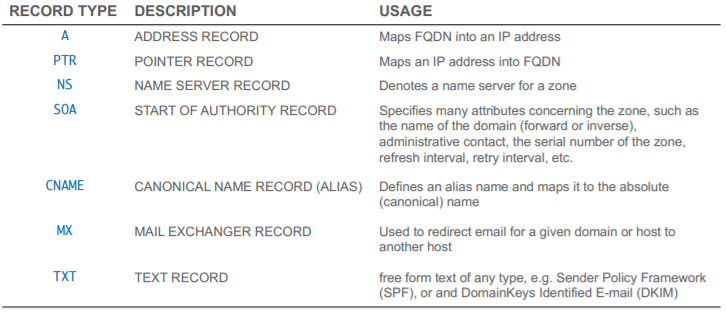
\includegraphics[scale=0.8]{images/915-rr.PNG}
	\caption{DNS resource record types.}
	\label{fig:rr}
\end{figure}

\paragraph{Attack Patterns}
Objective: insert tampered information into a DNS server or resolution process. See Figure \ref{fig:attack} for possible attacks on the DNS resolution process.

\begin{figure}[h]
	\centering
	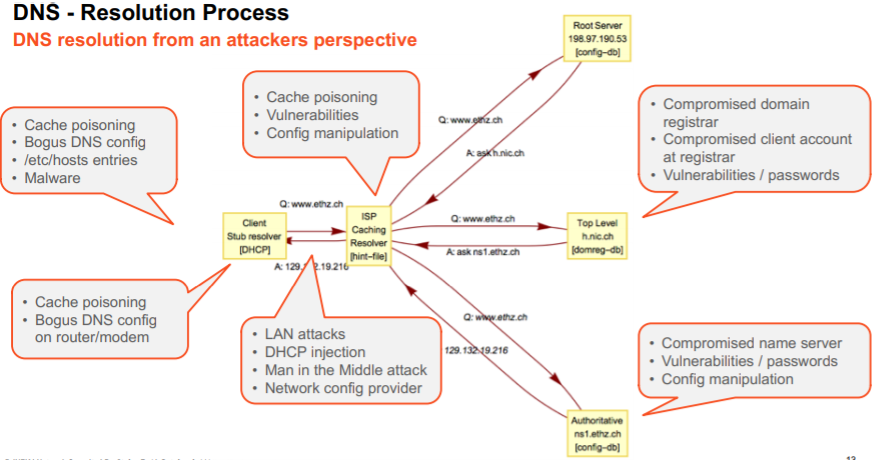
\includegraphics[scale=0.8]{images/915-attack.PNG}
	\caption{DNS resolution process from an attackers perspective.}
	\label{fig:attack}
\end{figure}

\paragraph{Common DNS Attacks}
\begin{itemize}
    \item \textbf{Local Host / Network:} Manipulate DNS entries and conversation on local host or network to impersonate services.
    \item \textbf{Cache Poisoning:} Inject manipulated information into DNS cache of resolver to impersonate services.
    \item \textbf{DNS Tunneling:} Use DNS as a covert communication channel to bypass firewalls to exfiltrate data and hidden communication.
    \item \textbf{DNS Hijacking:} Modify DNS record settings (often at domain registrar) to point to a rogue DNS server / domain to impersonate services.
    \item \textbf{Distributed Reflection:} Abuse a large number of DNS servers to combine reflection and amplification of queries that results in a (D)DoS attack.
\end{itemize}

\paragraph{DNS Root Server Security}
Served by 12 root server clusters (A to M) which are authoritative for queries for the top level domains. Every name resolution passes through this.

The root server system (RSS) consists of 1'342 instances and is operated by the 12 independent and diverse (globally and admin) root server operators (RSO). The primary concerns are availability and data integrity of the root zone.

To mitigate a (D)DoS attack on the network bandwidth level, hundreds of root servers are deployed accross different ISPs around the world and they're heavily anycasted.

To mitigate a (D)DoS attack on the memory / CPU level, the RSS is replicated and monitored. DNS enhancements pose a challenge (additional computational overhead).

\paragraph{Cache Poisoning}
Attacker inserts incorrect resolution information at any level of the resolution process (resolver, forwarder, etc.) and delays the reply of an authoritative name server (expensive lookup or DoS). 

It is basically a guessing game for the attacker. An attacker can force a server lookup for a domain (or multiple) and immediately send a number of fake replies that all guess the \textit{txid} and source port number of the request and include a redirect to a malicious IP.

E.g.: Vulnerability patched in 1997 - exploiting the additional section field. By tricking a client to resolve a malicious domain (attacker owns domain), the reply can include unrelated information in an \textit{additional section} field for another valid domain which is then accepted and cached.

E.g.: SADDNS Attack. By forcing a server to send out a query, its source port is public info. Using a port scanner, one can identify the open port (dropped packet = open port, else ICMP port unreachable). Once identified, send large number of spoofed DNS replies to bruteforce \textit{txid} (all while delaying the legit response). %TODO: 2020 reload, overcoming ICMP rate limits, defenses

\paragraph{Compromised Configuration}
Attacking the domain registrar and making it provision wrong information. Second level domains are registered with one of the domain registrars of the top level domain. The DNS info is as secure as the webapp / registration processes / passwords of the registrar and the domain owner.

One can also manipulate the DNS configuration settings on an internal network or local host by attacking routers, attacking DHCP exchange, using malware to change local hosts file, etc.

%TODO: lessons learned?

\paragraph{DNS Security Extensions (DNSSEC)}
An extension to DNS introduced around 2000 (slow adoption) that provides origin authentication, authenticated denial of existence, integrity but neither availability nor data confidentiality. Zone data is digitally signed using a private key for that zone (parent signs children's public keys). A resolver only needs to know the root public key to authenticate DNS messages. Can have more (list of trust anchors) for zones it trusts implicitly.

To make this work, registrants that are responsible for publishing DNS information must ensure that their data is DNSSEC signed and network operators need to enable DNSSEC validation on their resolvers.

See Figure \ref{fig:dnssec} for some resource record types introduced by DNSSEC.

\begin{figure}[h]
	\centering
	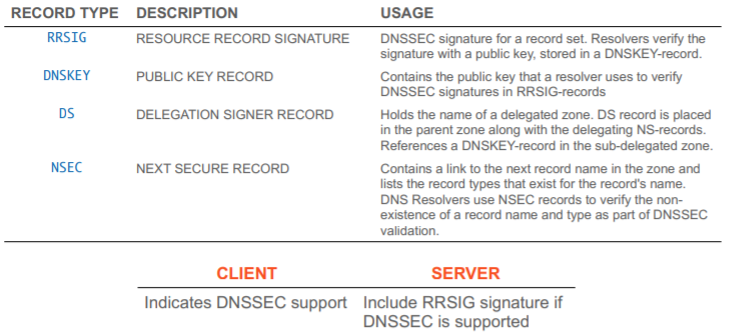
\includegraphics[scale=0.8]{images/915-dnssec.PNG}
	\caption{Resource record types added by DNSSEC.}
	\label{fig:dnssec}
\end{figure}

%TODO: disadvantages

\paragraph{DNS over HTTPS / TLS (DoH / DoT)}
Both protocols add confidentiality to DNS. Traditional DNS requests can be used to track a user. %TODO: more?


\paragraph{Conclusion}
\begin{itemize}
    \item DNS has suffered a feature creep, picking up increasingly more responsibilities.
    \item Ensure large enough randomness / entropy for critical fields.
    \item Consider impact of input validation, rate limiting, max. open / outstanding connections.
\end{itemize}
\newpage

\section{Mail Filtering}

\paragraph{Simple Mail Transfer Protocol (SMTP)}
Protocol used to send and receive mail messages. For clients, SMTP is used to send emails to a mail server for relaying. To retrieve messages, IMAP (retrieve mail from a mail server) or POP3 are used (or others / proprietary protocols).

Boundary MTA use DNS to look up the MX record for the recipient's domain (after @). MX record contains name of target MTA

\begin{figure}[h]
	\centering
	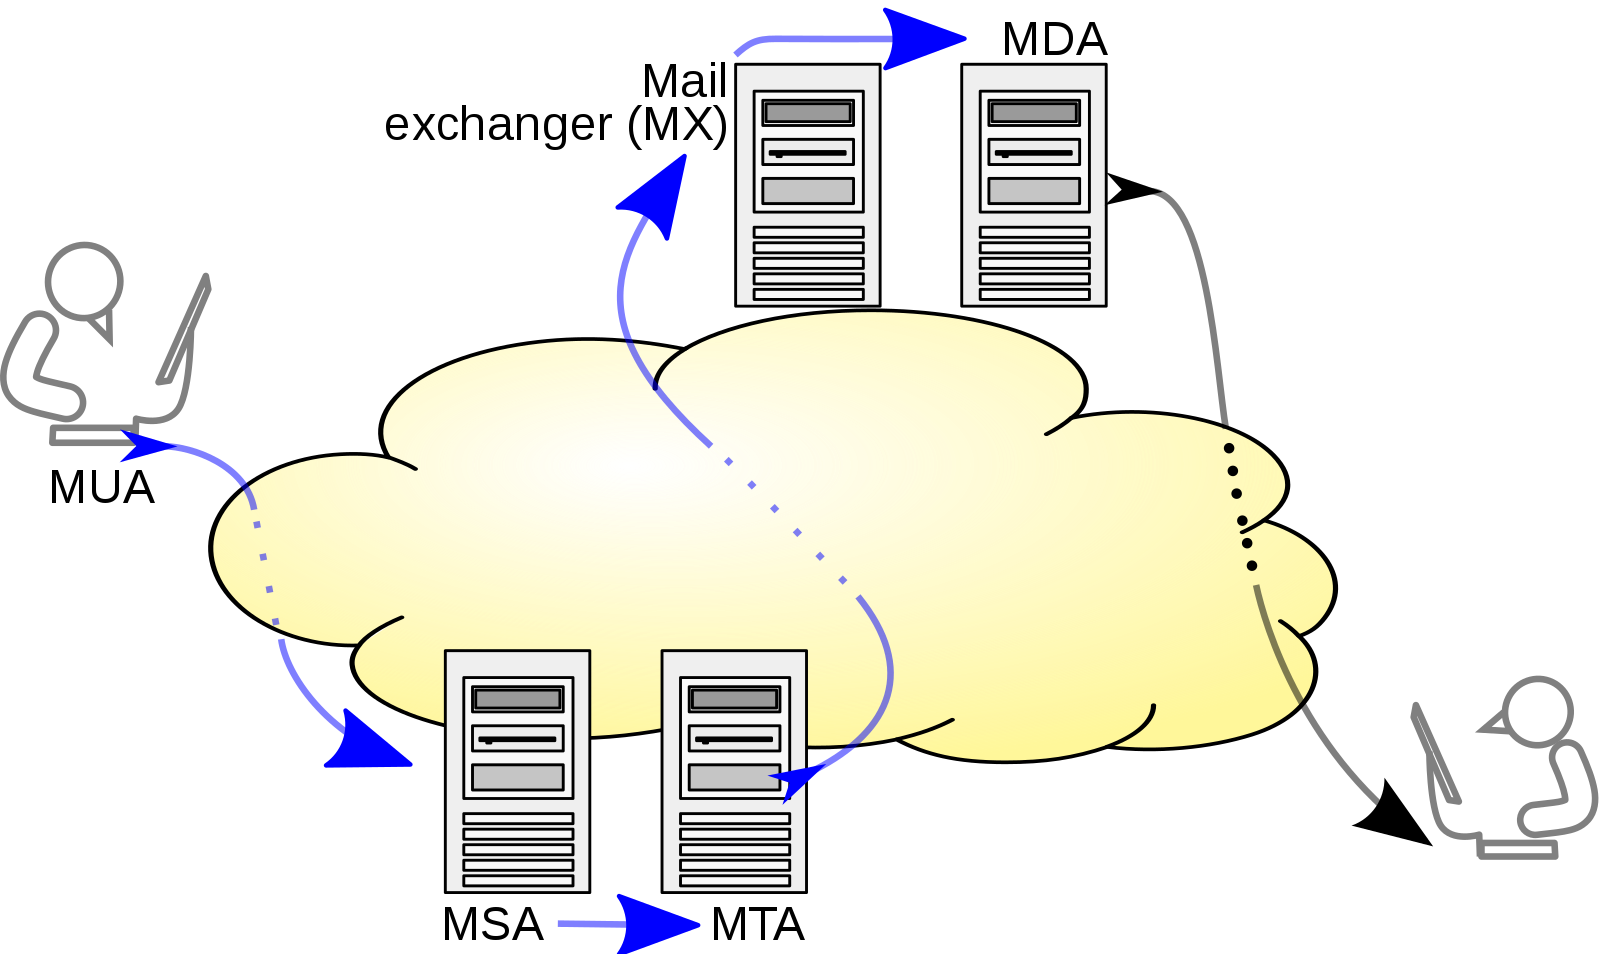
\includegraphics[scale=0.15]{images/916-smtp.png}
	\caption{Mail user agent sending an email to a mail submission agent, which in turn sends it to a mail transfer agent.}
	\label{fig:smtp}
\end{figure}

\begin{figure}[h]
	\centering
	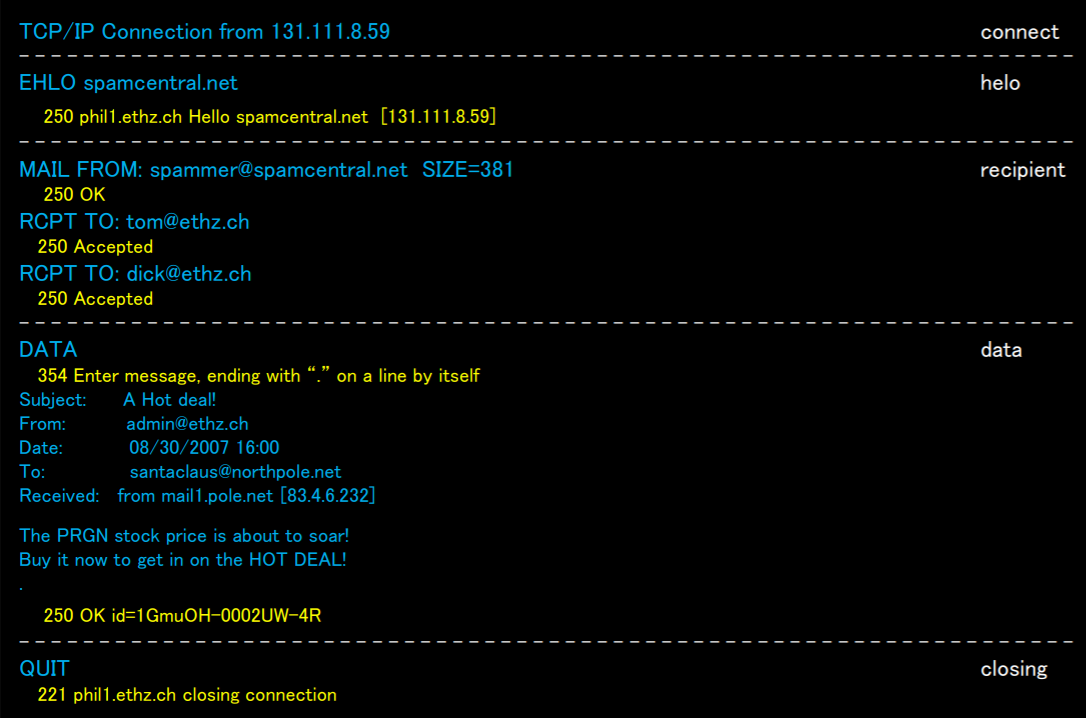
\includegraphics[scale=0.5]{images/916-session.PNG}
	\caption{Example of an SMPT message exchange. Note: actual sender and recipient does not match in message content.}
	\label{fig:session}
\end{figure}

\paragraph{Mail Filter}
There are several considerations when designing a mail filter:

\begin{itemize}
    \item Accept all and filter or already reject some during the SMTP session?
    \item Retrieve messages during a single SMTP session or multiple parallel ones?
    \item Filter only inbound mail or also outbound?
    \item Own DNS server for the filter?
    \item How to check valid recipient addresses? (local list, remote database, mail server, etc.)
    \item Will users have individual black- and whitelists?
    \item Will users have individual filtering preferences?
\end{itemize}
\newpage

\section{Probabilistic Traffic Monitoring}

%TODO: error rate?

\subsection{Overview}

\paragraph{Why Monitor Traffic}
Traffic monitoring can be used to detect anomalies (e.g. volume-based attacks such as a DoS or breaches of quality of service agreements) and to manage the network (usage-based pricing, traffic engineering, etc.).

Performed on a flow-based granularity. Flow = (Src IP, Dst IP, Src Port, Dst Port, Protocol). Also, IPv6 has an explicit flow label.

Difficult since there's so much traffic (and it grows fast) and packets needs to be processed in an extremely efficient manner.

\paragraph{Probabilistic Traffic Monitoring}
Trade accuracy (low bias) / precision (low variance) for efficiency by estimating traffic statistics based on actual traffic. 

\subsection{Measuring Flows}

\paragraph{General-Purpose Measurements (NetFlow)}
Standard NetFlow samples every packet, sampled NetFlow samples every k-th packet. It keeps a flow entry for each flow that counts the number of samples packets and bytes which is updated for every sample. To estimate the number of packets and bytes of a flow, the recorded values are multiplied by k.

\begin{figure}[h]
	\centering
	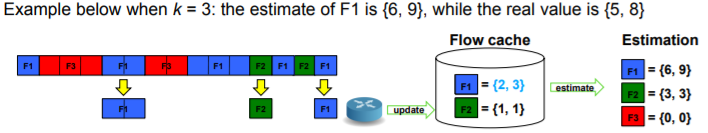
\includegraphics[scale=0.8]{images/917-netflow.PNG}
	\caption{Sampled NetFlow with k = 3.}
	\label{fig:netflow}
\end{figure}

Simple to implement and reduces the processing time but might be a memory overhead since there is one entry per flow in the worst case. The estimates are imprecise, especially for short-lived flows (most precise for flows sending many small packets). To solve imprecision, only focus on a specific traffic information instead of general purpose (e.g. only large flows as below, etc.)

\paragraph{Large Flows}
Flows that take up a given threshold of link capacity. E.g. hypergiants that generate 30\% of all Internet traffic. Less than 1\% of flows account for more than 90\% of traffic volume. It is easy to identify them (without keeping per-flow state on routers) because their number is much smaller than overall flows.

\paragraph{Sample and Hold}
Is a byte-sampling technique that takes packet size into account. Each byte is sampled with a probability $p$ so each packet with size $s$ is sampled with probability $p_s$ where $p_s = 1-(1-p)^s \approx p \cdot s$ (when $p$ is small). This reduces memory overhead since non-uniform sampling is biased toward large flows.

\begin{itemize}
    \item For each packet, check if its flow record exists. If yes, hold it (update flow entry). If no, sample it with probability $p_s$.
    \item Held / sampled packets are used to update the flow entries in the flow table (estimated number of packets and bytes per flow).
\end{itemize}

Comparison to NetFlow: Sample-and-Hold uses byte sampling instead of packet sampling. It does not over-count (but both might underestimate). Error rate of S-H is O($M^{-1}$) and of NF O($M^{-\frac{1}{2}}$) where $M$ is given memory overhead. S-H inspects all packet headers.

\paragraph{Single-Stage Filter}
Keep an array of $n$ counters. A router hashes the flow ID of an incoming packet with output $i$ in $\{1, ..., n\}$ and increases $i$-th counter. Flow is considered large if its counter value surpasses a threshold. To reduce false positives, use multiple filters in parallel.

\paragraph{Multistage Filter}
The above but with multiple filters in parallel, with each stage using a different independent hash function. Flow is large if all associated counter values surpass a threshold.

Uses fixed memory resources, no false negatives and low false positives (FP rate decreases exponentially in the number of stages).

\paragraph{Finding Frequent Items}
Find items (= packets) with a frequency that surpass chosen threshold (= large flow). See below for different kinds of algorithms.

\paragraph{Majority Algorithm}
Keep one item \textit{kept item} and one counter.

\textbf{First pass} For each new item: if counter equals to 0, \textit{kept item} is new item, increase counter, else if new item is same as \textit{kept item}, increase counter, else decrease counter.

\textbf{Second pass} Test the last \textit{kept item} to see if it is actually the one with >50\% frequency (majority).

\paragraph{MG-Algorithm}
Generalization of Majority Algorithm. Find all items that appear in a stream of $m$ items more than $k$ times with no false negatives and with limited space $n = \frac{m}{k} - 1$ counters. Needs a second pass to eliminate false positives (e.g. c in example).

\begin{figure}[h]
	\centering
	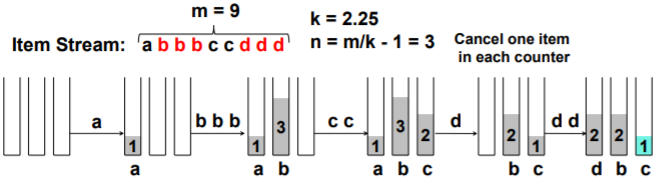
\includegraphics[scale=0.8]{images/917-mg.PNG}
	\caption{MG-algorithm.}
	\label{fig:mg}
\end{figure}

\paragraph{EARDet Algorithm}
Modifies the MG-Algorithm by switching number of packets with packet size and therefore increasing counter by size instead of number. Idle periods are replaced by virtual flows of a specific packet size (low-bandwidth threshold, e.g. idle period of 6 divided into two times 3 if THL is 3).

No false negatives for large flows and no false positives for small flows (if a certain threshold is surpassed by one of the items in the counter, it is frequent) - there is an ambiguity region between low-bandwidth and high-bandwidth threshold. Deterministic (keeps performance regardless of input traffic / attack pattern). Relatively small storage cost but many counters are needed. Con: per-packet counter is an expensive operation.

\begin{figure}[h]
	\centering
	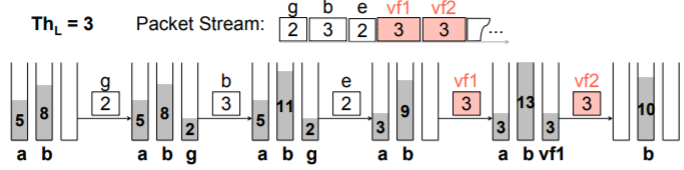
\includegraphics[scale=0.8]{images/917-eardet.PNG}
	\caption{EARDet algorithm.}
	\label{fig:eardet}
\end{figure}


\subsection{Finding Duplicates}

\paragraph{Problem}
Identify if an element is a duplicate without storing all previous elements. A Bloom Filter provides a probabilistic data structure for set membership testing.

\paragraph{Bloom Filter}
Start with bit vector $V$ that has $m$ bits and an initial value of 0. For each inserted element $e$, compute $k$ hash functions $h_i = H_i(e)$ where $0 < h_i \leq m$ and set all bits $V[h_i] = 1$. To test if an element $e'$ has already been seen, recompute all $k$ hash functions and check all $V[h_i]$, if all bits are 1, the element has been seen before.

No false negatives and constant time insertion / test. The more elements are inserted, the higher the probability of a false positive (reset filter, no more FN guarantee). Constant bits per element given FP rate (but still O(n) memory overhead).

%TODO: duplicates in practice

\begin{figure}[h]
	\centering
	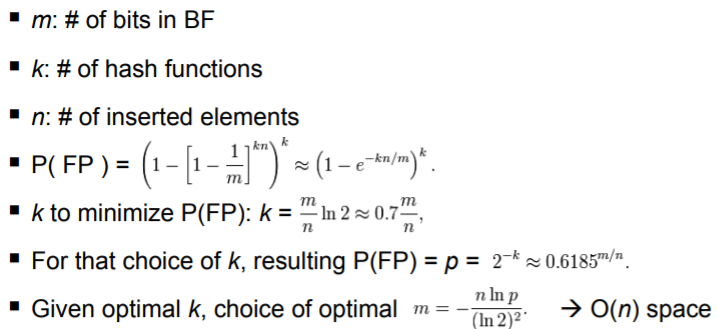
\includegraphics[scale=0.6]{images/917-bloom.PNG}
	\caption{Bloom Filter parameters.}
	\label{fig:bloom}
\end{figure}

\subsection{Estimate Number of Flows}

\paragraph{Probabilistic Counting}
See Figure \ref{fig:counting}. Problems: minimum can have very large variance and therefore this is not robust. An attacker controlling only one input can bias the estimation.

Proposal by Bar-Yossef et al.: keep track of the $k$ smallest hash values, expectation value of $k$-th smallest value is $\frac{k}{(n+1)}$ which has smaller variance. Estimate with $k$-th smallest value $v_k$ seen so far: $n \approx \frac{k}{v_k} - 1$.

Additionally, use sampling to reduce overhead induced by hashing.

\begin{figure}[h]
	\centering
	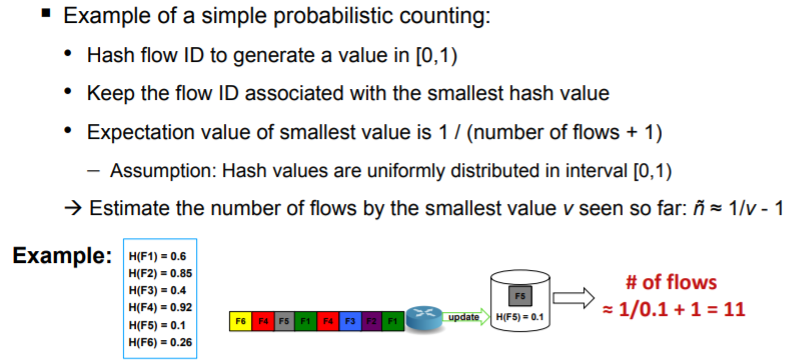
\includegraphics[scale=0.6]{images/917-counting.PNG}
	\caption{Probabilistic counting.}
	\label{fig:counting}
\end{figure}

%TODO: tm vs intrusion detection, challenges

\newpage

\section{Top N Ways to Get Domain Admin}

A field report from attack simulations across different companies.

Attacks exploit the human factor almost all of the time (e.g. phishing). You don't even need technical vulnerabilities. Just look for old and outdated stuff.

\paragraph{Attack Simulation}
The entire network is in scope (company and employees). We don't just test single groups or parts of the company network.
\newpage


\end{document}